%%%%%%%%%%%%%%%%%%%%%%%%%%%%%%%%%%%%%%%%%%%%%%%%%%%%%%%%%%%%
%
% This is the LaTeX version of DFG form 54.012 EN
%
%%%%%%%%%%%%%%%%%%%%%%%%%%%%%%%%%%%%%%%%%%%%%%%%%%%%%%%%%%%%

% DFG Bestaetigungsnummer: 20141001548940209703

\let\Div=\div
\renewcommand{\div}{\mathop{\mathrm{div}}}

\documentclass[enabledeprecatedfontcommands,cleardoublepage=empty,headsepline,twoside,11pt,DIV=15,BCOR=12mm,final]{scrartcl}
%twoside,
%\documentclass[twoside,11pt,]{scrartcl}\

\usepackage[colorlinks=true]{hyperref}
\usepackage[english]{babel}

\usepackage[right]{eurosym}
\usepackage{enumerate}

\usepackage{graphicx}

\usepackage{rotating,multirow,booktabs}

\usepackage{amsmath,amssymb}
\usepackage{comment,xspace}
\usepackage[latin1]{inputenc}
\usepackage{todonotes}
%\usepackage{color}
\usepackage{subfigure}
\usepackage[footsepline,headsepline]{scrpage2}
\usepackage{typearea}
\KOMAoptions{headsepline=true}
\KOMAoptions{footsepline=true}
\KOMAoptions{cleardoublepage=empty}


\newcommand{\note}[1]{\marginpar{%
    \fbox{\begin{minipage}{25mm}
       #1
    \end{minipage}}}}

\newcommand{\newf}[1]{}%{\color{red}{#1}}}

\newcommand\todoin[2][]{\todo[inline, caption={2do}, #1]{
 \begin{minipage}{\textwidth-4pt}#2\end{minipage}}}

\ohead{\textsf{\pagemark}}
\ofoot{\textsf{DFG Application ``Adaptive Finite Element Methods for Total Variation Minimization''}}
\cfoot{}

\renewcommand{\titlepagestyle}{empty}

\usepackage[labeled]{multibib}
\newcites{A,B}%
{{Articles published by outlets with scientific quality assurance, book publications, and works accepted for publication but not yet published},{Other publications}}



\renewenvironment{description}
{\begin{list}{\epdes}{\topsep0mm \labelwidth0mm \leftmargin3mm %
  \itemsep1pt plus 4pt \topsep3pt \parsep1pt plus 4pt \labelsep3mm}}
{\end{list}}
\renewenvironment{itemize}
{\begin{list}{$\triangleright$}{\labelwidth-2mm \leftmargin3mm %
  \itemsep5pt plus 0pt  \topsep3pt \parsep1pt plus 4pt \labelsep2mm}}
{\end{list}}

% for having several reference lists...
\newcounter{savecount}
\newcommand{\ourbibitem}[1]{%
\stepcounter{savecount}\def\ourlabel{O\arabic{savecount}}\bibitem[\ourlabel]{#1}}


% a, A
\newcommand{\As}[1][s]{\ensuremath{\mathbb{A}_{#1}}}
\newcommand{\abs}[1]{\ensuremath{\left|#1\right|}}
\newenvironment{algotab}%
{~\ttfamily\begin{samepage}%
\begin{tabbing}%
 \hspace*{5mm}\=\hspace{3ex}\=\hspace{3ex}\=\hspace{3ex}\=\hspace{3ex}%
\=\hspace{3ex}\=\hspace{3ex}\=\hspace{3ex}\=\hspace{3ex}\kill}%
{\end{tabbing}\end{samepage}}
\newcommand{\astfem}{\textsf{ASTFEM}\xspace}
\newcommand{\alberta}{\textsf{ALBERTA}\xspace}
% b, B

\newcommand{\B}{\mathcal{B}}
\newcommand{\bilin}[2]{\B[#1,\,#2]}

% c, C
\newcommand{\C}{{\mathbb C}}
\newcommand{\cGq}[1][q]{\textsf{cG$(#1)$}\xspace}
\newcommand{\Cleq}{\ensuremath{\lesssim}}
\newcommand{\Cgeq}{\ensuremath{\gtrsim}}
% d, D
\newcommand{\definedas}{\mathrel{:=}}
\newcommand{\dGq}[1][q]{\textsf{dG$(#1)$}\xspace}
\newcommand{\DOF}{\textsf{DOF}\xspace}
\newcommand{\DOFs}{\textsf{DOFs}\xspace}
\newcommand{\dual}[3][]{\ensuremath{\langle #2,\, #3\rangle}_{#1}}
\newcommand{\dt}{{\rm d}t\xspace}
\newcommand{\dune}{\textsf{DUNE}\xspace}
\newcommand{\dunefem}{\textsf{DUNE-FEM}\xspace}

% e, E
\newcommand{\E}{{\mathbb E}}
\newcommand{\elm}{E}
\newcommand{\epde}{\textsf{ePDE}\xspace}
\newcommand{\epdes}{\textsf{ePDEs}\xspace}

% g, G
\newcommand{\grid}{\mathcal{G}}
\newcommand{\G}{\mathbb{G}}

% h, H
\newcommand{\helm}[1][\elm]{\ensuremath{h_{#1}}}

% i, I
\newcommand{\ie}{i.\,e.}

% n, N
\newcommand{\N}{{\mathbb N}}

% P, p
\newcommand{\ppde}{\textsf{pPDE}\xspace}
\newcommand{\ppdes}{\textsf{pPDEs}\xspace}

% Q, q
\newcommand{\Q}{{\mathbb Q}}

% r, R
\newcommand{\R}{{\mathbb R}}

% t, T
\newcommand{\Tn}[1][n]{\ensuremath{\mathcal{T}_{#1}}}
\newcommand{\taun}[1][n]{\ensuremath{\tau_{#1}}}
\newcommand{\tol}{\textsf{TOL}\xspace}

% u, U
\newcommand{\Un}[1][n]{\ensuremath{U_{#1}}}

% v, V
\newcommand{\V}{\ensuremath{\mathbb{V}}}
\newcommand{\VN}[1][N]{\ensuremath{\V_{\!#1}}}

% w, W
\newcommand{\W}{\ensuremath{\mathbb{W}}}
\newcommand{\WN}[1][N]{\ensuremath{\W_{\!#1}}}
\newcommand{\Wclass}{\ensuremath{\mathcal{W}}}

% z, Z
\newcommand{\Z}{{\mathbb Z}}



\newcommand{\bnew}[1]{\textcolor{blue}{#1}}



\newcommand{\sbt}{\,\begin{picture}(-1,1)(-1,-3)\circle*{2}\end{picture}\ }






\begin{document}

\begin{titlepage}\sffamily
  \subject{DFG Research Grant Application} 
  \title{Adaptive Methods for Free Discontinuity Problems}% (for Image Reconstruction)}
  
  \author{Andreas Langer and Fernando Gaspoz}
  \date{Stuttgart, \today \\[50mm] Submission\\[50mm]
    Application period: 01.01.2019 --- 31.12.2021}
\end{titlepage}

\maketitle[-1]
\cleardoublepage
\setcounter{page}{1}
\pagestyle{scrheadings}


\section*{Applicants}

\subsection*{Principle Investigator}

\begin{flushleft}
  \textbf{Dr. Andreas Langer}
  \begin{tabbing}
    DFG reference number:\quad\=Phone:\quad\=\kill
    Position:\> Deputy Professor\\% PostDoc\\
    %DFG reference number:\>SI 814/1-2\\[1mm]
    Contact:\> Numerische Mathematik f\"ur H\"ochstleistungsrechner\\ 
    \>Institut f\"ur Angewandte Analysis und Numerische Simulation\\
    \> Universit\"at Stuttgart\\
    \> Pfaffenwaldring 57 \\
    \> D-70569 Stuttgart\\[1mm]
    \> Email:\> andreas.langer@ians.uni-stuttgart.de\\[1mm]
 \end{tabbing}
\end{flushleft}


\begin{flushleft}
  \textbf{Dr. Fernando Gaspoz}
  \begin{tabbing}
    DFG reference number:\quad\=Phone:\quad\=\kill
    Position:\> PostDoc\\
    %DFG reference number:\>SI 814/1-2\\[1mm]
    Contact:\> Numerische Mathematik f\"ur H\"ochstleistungsrechner\\ 
    \>Institut f\"ur Angewandte Analysis und Numerische Simulation\\
    \> Universit\"at Stuttgart\\
    \> Pfaffenwaldring 57 \\
    \> D-70569 Stuttgart\\[1mm]
    \> Email:\> fernando.gaspoz@ians.uni-stuttgart.de\\[1mm]
 \end{tabbing}
\end{flushleft}

\subsection*{Co-Investigator}

\begin{flushleft}
  \textbf{Prof. Dr. Kunibert G. Siebert}
  \begin{tabbing}
    DFG reference number:\quad\=Phone:\quad\=\kill
    Position:\> Professor\\
    %DFG reference number:\>SI 814/1-2\\[1mm]
    Contact:\> Numerische Mathematik f\"ur H\"ochstleistungsrechner\\ 
    \>Institut f\"ur Angewandte Analysis und Numerische Simulation\\
    \> Universit\"at Stuttgart\\
    \> Pfaffenwaldring 57 \\
    \> D-70569 Stuttgart\\[1mm]
    \> Email:\> kunibert.siebert@ians.uni-stuttgart.de\\[1mm]
 \end{tabbing}
\end{flushleft}
\section*{Project Description}

\paragraph{Summary.} 

In many modern applications, like image reconstruction and image analysis, the solution of interest is described by a discontinuous function. Unfortunately, it is a priori not known where the discontinuities  are located and that has to be determined numerically. In fact, computing discontinuities wrongly or inaccurately could be either fatal (as in obstacle and tumor detection) or scientifically costly.  %One approach is to optimize a functional, which consists of a generalized, measure-valued, gradient term.
In order to preserve edges and discontinuities  in image processing, the minimization of a functional consisting of a the total variation term is common and widely used. Typical applications, where such a optimization problem is solved are for example: image denoising, image inpainting, and the determination of motion in image sequences. Note that all these examples are ill-posed inverse problems and hence the optimization problem is originated by regularization techniques, e.g., total variation regularization.

In this project we solve the constituted problems by constructing methods, which automatically adjust to the discontinuities of the underlying (observed) data. This adjustment leads to methods, which adaptively (in an iterative manner) reduce the reconstruction error, allowing to obtain the discontinuities more accurately and hence yield qualitatively better reconstructions, and reduce the computational complexity of the underlying problem at the same time. Additionally to these attributes the derived methods will possess further desirable properties, as robustness with respect to the given data, they are guaranteed to converge to a more accurate solution than state-of-the-art methods, and they allow for different discretisation techniques. 

The adaptive adjustment of the derived methods occur on two sides, on the regularization side, where the regularization is locally adjusted, and on the discretization side, where an optimal discretization is learned. We derive criteria based on edge-indicators, a posteriori estimates and local residuals, which tell us, how the adjustment of the regularization and discretization should be performed. In particular, at discontinuities the regularization should be very small, preventing any smoothing, while the mesh should be very fine, allowing for depicting the discontinuities very precisely. 

In this vein, these adaptive methods are especially important in real-world applications, where the solution needs to be computed accurately, as they allow for a very precise solution while keeping the computational complexity on a manageable level. With the proposed research we will substantially foster the development and numerical analysis of optimal adaptive methods for non-smooth inverse imaging problems. %In addition, the investigation will contribute to a better understanding of the used models and their respective solvers.

%We will mainly focus on two aspects of adaptivity. Firstly we consider an adaptive discretization of the underlying problem. Note, that adaptive finite elements are well understood for (elliptic) partial differential equations and have gained a lot of attention. They have been used in numerous practical applications showing very robust performance. Convergence proofs and optimal decay rates in terms of degree of freedom are available. We will design and analyse adaptive finite element methods for non-smooth variational image models. In particular, we will develop an adaptive discretization environment for the reconstruction of only partly given images (image inapinting) and for determining motion in image sequences. These challenging topics require the investigation of appropriate finite element discretization and a posteriori estimates. 

%Secondly we will consider an adaptive regularization of the ill-posed inverse imaging problems.

The principal investigators and co-investigator have a long track record in research areas like mathematical image processing, inverse problems, non-smooth optimisation, finite element methods, a posteriori estimates and adaptive methods. Furthermore, several mathematical problems involved in the project are quite suitable for postgraduate training.


%  analyze finite element methods for the minimization of the non-smooth and non-additive total variation with main focus on adaptive discretization.

%In order to preserve edges and discontinuities in images, in image reconstruction the minimization of a functional consisting of a the total variation term is common and widely used. Typical applications, where such a optimization problem is solved, are for example image denoising, image inpainting, and image deblurring. Due to better hardware in such applications one has to deal with high-dimensional images and data sets. Since most of the images have very uniform parts, a way to reduce the number of picture elements is to discretize by the use of different sizes of picture elements, i.e., using adaptive finite elements.

%Adaptive finite elements are well understood for (elliptic) partial differential equations and have gained a lot of attention. They have been used in numerous practical applications showing very robust performance. Convergence proofs and optimal decay rates in terms of degree of freedom are available.

%Real world applications in image reconstruction would tremendously profit from an adaptive discretization environment. However, the understanding of how to use adaptive finite elements as well as the analysis of respective methods in particular for non-smooth variational image reconstruction, is yet, in our opinion, in a very early stage. There exist only first approaches for clean images and image denoising of Gaussian noise.

%The proposed research project focuses on the design and analysis of adaptive finite element methods for non-smooth variational image reconstruction. We will develop an adaptive environment for the reconstruction of images containing a mixture of noise. Note, that in real world applications images are usually corrupted by more than one type of noise. This challenging topic requires the investigation of appropriate finite element discretization and a-posteriori estimates. 

%With the proposed research we will substantially foster the development and numerical analysis of optimal adaptive methods for non-smooth minimization problems for image reconstruction. In addition, the investigation will contribute to a better understanding of the used models and their respective solvers.

\section{State of the art and preliminary work}
\label{sec:state-prelim}

\subsection{State of the art}
\label{sec:state} 

\subsubsection{Free discontinuity problems}

In certain applications, the desired solution should contain discontinuities, whereas it is a priori not know at which locations they will occur. Typical examples of such applications are found in image reconstruction, image analysis, and material science. In image reconstruction one is interested in recovering an image from its observed corrupted data, whereas the corruption might be for example noise or missing parts. Image analysis addresses the task of analysing the given observation. Here one might be for example interesting in extracting or detecting certain features or objects in an image. In case of image sequences also the question of detecting the motion of certain objects is part of image analysis. In material science a typical example is the calculation of the propagation of a crack path. In all these applications, in order to allow for a discontinuous solution, one usually minimizes a functional consisting of a total variation term. We recall, that for $u\in L^1(\Omega)$, where $\Omega \subset \R^2$ is a bounded open domain with Lipschitz boundary,
$$
V(u,\Omega):=\sup\left\{\int_{\Omega} u \operatorname{div} \phi \ \text{d}x : \phi \in [C_c^1(\Omega)]^2, \|{\phi}\|_{L^\infty(\Omega)} \leq 1\right\}
$$
is the variation of $u$ in $\Omega$. Here, $L^q(\Omega)$, with $q\in [1,\infty]$, denotes the usual Lebesgue space \cite{AdaFou} and $C_c^l(\Omega)$, $l\in \N$, is the space of $l$-times continuously differentiable functions with compact support in $\Omega$. In the event that $V(u,\Omega)<\infty$ we denote $|Du|(\Omega)=V(u,\Omega)$ and call it the total variation of $u$ in $\Omega$; see \cite{AmbFusPal, Giu} for more details. If $u\in W^{1,1}(\Omega)$, then $|Du|(\Omega)= \int_{\Omega}|\nabla u| dx$. Further, $BV(\Omega)$ denotes the space of functions with bounded variation, i.e., $u\in BV(\Omega)$ if and only if $V(u,\Omega)<\infty$. The space $BV(\Omega)$ endowed with the norm $\|u\|_{BV} = \|u\|_{L^1(\Omega)} + |Du|(\Omega)$ is a Banach space \cite{Giu}. 

\paragraph{Image reconstruction}

In image restoration one is interested in recovering an unknown image from a corrupted observation. Hence, the obtained data $g$ might be described as
$$
g=\mathcal{N}(T\hat{u}),
$$
where $\hat{u}$ is the unknown original image, $T$ is a linear bounded operator modeling the image formation device, and $\mathcal{N}$ represents noise. %In this project we will concentrate on images, which do not possess any noise or they are corrupted by Gaussian noise. 
We note, that in reality in general not only one type of noise, but a mixture of several different types, such as Gaussian, Poisson, and impulse noise, occur in an image. This contamination usually happens during image acquisition and image transmission. Nevertheless, in case the image is not effected by impulse noise, the mixture of Gaussian and Poisson noise can be transformed into additive white Gaussian noise \cite{}. In this vein, we will mainly focus in this project on either  Gaussian noise corrupted images or images which are noise-free at all. However, we plan to extend the work to other types of noise as well, by noting that this leads to different models, see below, and hence to a different analysis and numerical implementation. \todo{really or extend to more types of noise?}

Due to the action of $T$, even in the noise-free case the reconstruction of $\hat{u}$ from $g$ is usually an ill-posed inverse problem and thus regularization techniques are required \cite{EngHanNeu}. A good approximation may be obtained by minimizing a functional consisting of a data term, which enforces the consistency between the recovered and measured image, a regularization term to prevent over-fitting, and a parameter $\lambda>0$ weighting the importance of these two terms. Since we are aiming at preserving discontinuities and edges in an image, the total variation is typically chosen as a regularization technique. However, we note, that a more sophisticated regularizer, as the nonlocal total variation \cite{KinOshJon}, the total generalized variation \cite{BreKunPoc}, a higher order regularizer (see e.g. \cite{PapSch} and references therein), or a nonconvex regularizer might be used as well \cite{}. %\todo{Nonconvex regularizer, $\ell^p$, $0<p<1$} Nevertheless, for simplicity in the sequel of this section we will only consider total variation regularisation, but we keep in mind that other regularisers might be used as well, possibly rendering the problem more complicated. 
In the application of image inpainting, we will consider in this project, for example, a higher order regularizer, leading to the following minimization problem proposed in \cite{EseShe} %e.g., %$\gamma \int_{\Omega\setminus K} |\nabla u(x) |^2 \text{d}x + \int_K (\lambda + \beta \kappa^2) \text{d}s$, where $\Omega\subset \R^2$ is the image domain, $\gamma,\lambda, \beta \in \R_+$, and $K$ represents the edges of the image $u$.
 %the minimization problem proposed in \cite{EseShe}
\begin{equation}\label{Eq:MSInpainting}
\min_{u,K} \int_{\Omega\setminus K} |\nabla u(x) |^2 \text{d}x + \lambda \mathcal{H}^1(K) + \beta \int_K \kappa^2 + \alpha \int_\Omega |\chi_{\Omega\setminus K}(x) u(x) - g(x)|^2 \text{d}x,
\end{equation}
where $\Omega\subset \R^2$ is the image domain, $g\in L^\infty(\Omega)$ is the observation, $\alpha,\beta,\lambda\in \R_+$ are parameters, $\kappa$ denotes the curvature, and $K$ represents the edges of the image $u$. In particular, $K$ is a set of Hausdorff one-dimensional measure $\mathcal{H}^1(K)$.
%where $\beta > 0$ is a parameter and $\kappa$ represents the curvature, is considered.
Note that the minimization of \eqref{Eq:MSInpainting} is difficult, due to a minimization over $u$ and $K$ rendering the problem non-convex. In order to solve this problem, one may use the approximation based on  the work  \cite{AmbTor}. This approach is justified through $\Gamma$-convergence and approximates the edge set $K$ by some smooth function, rendering the problem easier to solve practically. 

The choice of the data-term typically depends on the type of noise contamination. For Gaussian noise contaminated images a quadratic $L^2$-data-term is usually chosen and has been successfully used; see for example \cite{Cha, ChaDar, ChaLio, ChaGolMul, ComWaj, DarSig05, DarSig06, DauTesVes, DobVog, GolOsh, HinSta, Nes, OshBurGolXuYin, WeiBlaAub}. In this case, which we refer to as the $L^2$-model, an approximation of the unknown original image $\hat{u}$ is obtained for the observed data $g$ by solving 
\begin{equation}\label{L2TV}
\min_{u\in BV(\Omega)} \|Tu-g\|_{L^2(\Omega)}^2 + \lambda R(u),
\end{equation}
where $T : L^2(\Omega) \to L^2(\Omega)$ is a bounded linear operator modelling the image-formation device and $R$ represents the regularizer. If $R(u)=\int_\Omega |Du|$, then we call \eqref{L2TV} the $L^2$-TV model. In case the image is only corrupted by noise one typically sets $T=I$. For image inpainting the observed image has missing parts $D\subset \Omega$, and hence $T$ is set to be the characteristic function of $\Omega\setminus D$, i.e., $Tu=\chi_{\Omega\setminus D}\cdot u$. \todo{Other relevant choices of $T$}%in case the observed image is blurry, $T$ represents the respective convolution (blurring) operator. 
 Here and in the sequel we assume that $T$ is known.

In connection with other type of noise models, other and different fidelity terms have been considered, see for example \cite{} for impulse noise, \cite{} for Poisson noise, \cite{} for multiplicative noise, and \cite{} for Rician noise.

\paragraph{Image analysis}

Image analysis addresses the task of analysing the given observation. Here we will concentrate on  the computation of optical flow only. 
%Image segmentation deals with the partitioning (or segmentation) of the image domain into different regions. Thereby the separation should be performed in a meaningful way, for example, that different objects depicted in an image are segmented and detected. In order to solve the image segmentation problem, one may solve the following optimization problem, proposed by Mumford and Shah \cite{MumSha},
%\begin{equation}\label{Eq:MSProblem}
%\min_{u,K} \left\{\mathcal{G}(u,K):= \int_{\Omega\setminus K} |\nabla u(x) |^2 \text{d}x + \lambda \mathcal{H}^1(K) + \alpha \int_\Omega |u(x)-g(x)|^2 \text{d}x\right\},
%\end{equation}
%where $\Omega\subset \R^2$ is the image domain, $g\in L^\infty(\Omega)$ is the observation, $\alpha,\lambda\in \R_+$ are parameters, and $K$ represents the edges of the image $u$. In particular, $K$ is a set of Hausdorff one-dimensional measure $\mathcal{H}^1(K)$. In case $\alpha=0$, problem \eqref{Eq:MSProblem} can be also used to predict quasi-static crack evolution \cite{FraMar}.  An extension of \eqref{Eq:MSProblem} to solve the problem of image inpainting is presented in \cite{EseShe}, i.e.,
%\begin{equation}\label{Eq:MSInpainting}
%\min_{u,K} \int_{\Omega\setminus K} |\nabla u(x) |^2 \text{d}x + \lambda \mathcal{H}^1(K) + \beta \int_K \kappa^2 + \alpha \int_\Omega |\chi_{\Omega\setminus D}(x) u(x) - g(x)|^2 \text{d}x,
%\end{equation}
%where $\beta > 0$ is a parameter and $\kappa$ represents the curvature, is considered.
%
%Note that the minimization of $\mathcal{G}$ and \eqref{Eq:MSInpainting} are difficult, due to a minimization over $u$ and $K$rendering the problem non-convex. In order to solve the image segmentation problem, several approximations of \eqref{Eq:MSProblem} have been proposed, see for example \cite{AubKor} and references therein. The most prominent approximation is probably the one proposed by Ambrosio and Tortorelli \cite{AmbTor}. This approach is based on $\Gamma$-convergence and approximates the edge set $K$ by some smooth function, rendering the problem easier to solve practically. This approximation strategy has also been applied in \cite{EseShe} to practically solve \eqref{Eq:MSInpainting}. 
%The second application we are concerned with according to image analysis is 
The estimation of motion is a crucial task in many applications. For example in the development of self-driving cars, it is a very important aspect that the vehicle itself is able to recognize danger and, consequently,  to react accordingly (artificial intelligence). In order to detect dangers, the motion of objects in the surrounding needs to be determined. One possibility is to record the surrounding as images, or better as a sequence of images. From these images the motion of the objects needs to be extracted. However, images do not record the actual motion, but only the projection of the motion into the 2D image plane. That is, one spatial component gets lost. Hence, from the image sequence we are able to determine the apparent motion, called \emph{optical flow}. By ``apparent'' we mean, that the motion can only be observed by the change of the intensity in a pixel. 

A common and widely used method to link the intensity change with the motion is the \emph{optical flow constraint}. Thereby it is assumed that the intensity $u(x,t)$ in $x\in \Omega$ along its trajectory $x(t)$ keeps constant. Such an assumption is reasonable for small changes, as long as no superposition appears. Let $\frac{\text{d}x}{\text{d}t}=v(x,t)$, by $\frac{\text{d}u}{\text{d}t}=0$ the optical flow constraint is
\begin{equation}\label{Eq:OFC}
u_t(x,t) + \nabla u(x,t) \cdot v(x,t) = 0.
\end{equation}
Unfortunately, one scalar equation is not enough to compute both components of the motion field $v=(v_1,v_2)^T$. Hence, in general there exist infinity many solutions and the problem is ill-posed. As in the case of image reconstruction regularization techniques are required to solve the problem. Since the optical flow is in general discontinuous and possesses jumps, a commonly used model, to compute an approximation of the motion field, solves a problem of the type \eqref{L2TV}, where $T=(\partial_x u, \partial_y u)\cdot $, $g=-u_t$, and $R(u)=\int_\Omega |Du|$ \cite{AubDerKorn1999,AubKor}.
\todo{maybe also describe mass-preserving constraint}



%\paragraph{The total variation model}
%In image restoration one is interested in recovering an unknown image from a corrupted observation. This recovery is usually an ill-posed inverse problem and thus regularization techniques are required \cite{EngHanNeu}. A good approximation may be obtained by minimizing a functional consisting of a data term, which enforces the consistency between the recovered and measured image, a regularization term to prevent over-fitting, and a parameter $\alpha>0$ weighting the importance of these two terms. In \cite{ROF} the total variation was introduced as a regularization technique in image reconstruction and has received considerable attention in image processing since then. We recall, that for $u\in L^1(\Omega)$, where $\Omega \subset \R^2$ is a bounded open domain with Lipschitz boundary,
%$$
%V(u,\Omega):=\sup\left\{\int_{\Omega} u \operatorname{div} \phi \ \text{d}x : \phi \in [C_c^1(\Omega)]^2, \|{\phi}\|_{L^\infty(\Omega)} \leq 1\right\}
%$$
%is the variation of $u$ in $\Omega$. Here, $L^q(\Omega)$, with $q\in [1,\infty]$, denotes the usual Lebesgue space \cite{AdaFou} and $C_c^l(\Omega)$, $l\in \N$, is the space of $l$-times continuously differentiable functions with compact support in $\Omega$. In the event that $V(u,\Omega)<\infty$ we denote $|Du|(\Omega)=V(u,\Omega)$ and call it the total variation of $u$ in $\Omega$; see \cite{AmbFusPal, Giu} for more details. If $u\in W^{1,1}(\Omega)$, then $|Du|(\Omega)= \int_{\Omega}|\nabla u| dx$. Further, $BV(\Omega)$ denotes the space of functions with bounded variation, i.e., $u\in BV(\Omega)$ if and only if $V(u,\Omega)<\infty$. The space $BV(\Omega)$ endowed with the norm $\|u\|_{BV} = \|u\|_{L^1(\Omega)} + |Du|(\Omega)$ is a Banach space \cite{Giu}. Note, that natural and man-made images may be characterized by edges and relatively uniform parts. Since the total variation is able to preserve edges and discontinuities in images, it seems suitable to us to use it as the regularization term. However, we note that a more sophisticated regularizer, as the nonlocal total variation \cite{KinOshJon}, the total generalized variation \cite{BreKunPoc}, or a higher order regularizer (see e.g. \cite{PapSch} and references therein) might be used as well.
%
%The choice of the data-term typically depends on the type of noise contamination. Usually images are corrupted by different types of noise, such as Gaussian noise and impulse noise. This contamination usually happens during image acquisition, which describes the process of capturing an image by a camera and converting it into a measurable entity \cite{Moe}, and image transmission. For images corrupted solely by Gaussian noise a quadratic $L^2$-data-term is usually chosen and has been successfully used; see for example \cite{Cha, ChaDar, ChaLio, ChaGolMul, ComWaj, DarSig05, DarSig06, DauTesVes, DobVog, GolOsh, HinSta, Nes, OshBurGolXuYin, WeiBlaAub}. In this case, which we refer to as the $L^2$-TV model, an approximation of the unknown original image $\hat{u}$ is obtained for the observed data $g$ by solving 
%\begin{equation}\label{L2TV}
%\min_{u\in BV(\Omega)} \alpha \|Tu-g\|_{L^2(\Omega)}^2 + |Du|(\Omega),
%\end{equation}
%where $T : L^2(\Omega) \to L^2(\Omega)$ is a bounded linear operator modeling the image-formation device. For example, in case the observed image is blurry, $T$ represents the respective convolution (blurring) operator. If the image is only corrupted by noise one sets $T=I$. Here and in the sequel we assume that $T$ is known.
%
%The $L^2$-TV model usually does not yield a satisfactory restoration in the presence of impulse noise. This type of noise is usually constituted due to malfunctioning pixels in camera sensors, faulty memory locations in hardware, or transmission over noisy digital links. There are two commonly used models of impulse noise considered in the literature. The first one, called \emph{salt-and-pepper noise}, where the noisy image $g$ is given by
%$$
%g(x) = 
%\begin{cases}
%d_{\min} & \text{ with probability } s_1\in [0,1),\\
%d_{\max} & \text{ with probability } s_2\in [0,1),\\
%T \hat{u}(x)  & \text{ with probability } 1-s_1-s_2,
%\end{cases}
%$$
%with $1-s_1-s_2>0$ \cite{ChaHoNik}. Here and in the rest of the paper we assume that $T \hat{u}$ is in the dynamic range $[d_{\min},d_{\max}]$, i.e., $d_{\min}\leq T\hat{u}\leq d_{\max}$. The second model is called \emph{random-valued impulse noise}, where $g$ is described as
%$$
%g(x) = 
%\begin{cases}
%c & \text{ with probability } s\in [0,1),\\
%T \hat{u}(x)  & \text{ with probability } 1-s,
%\end{cases}
%$$
%with $c$ being a uniformly distributed random variable in the image intensity range $[d_{\min},d_{\max}]$. For impulse noise contaminated images a more successful approach uses instead of a quadratic $L^2$-data-fidelity term a non-smooth $L^1$-data-fidelity term \cite{All, Nik2002, Nik2004}. That is, instead of \eqref{L2TV} one optimizes the following minimization problem
%\begin{equation}\label{L1TV}
%\min_{u\in BV(\Omega)} \alpha \|Tu-g\|_{L^1(\Omega)} + |Du|(\Omega),
%\end{equation}
%which we call the $L^1$-TV model. 
%
%We are interested in recovering images, which are contaminated by a mixture of Gaussian and impulse noise. Recently in \cite{HinLan2013} an $L^1$-$L^2$-data-fidelity term has been introduced and shown to be suited to the task of removing mixed Gaussian-impulse noise. In this approach, which we call $L^1$-$L^2$-TV model, an image is restored by solving
%\begin{equation}\label{L1L2TVmodel}
%\min_{u\in BV(\Omega)} \alpha_1 \|T_1u-g_1\|_{L^1(\Omega)} +  \alpha_2 \|T_2 u-g_2\|_{L^2(\Omega)}^2 + |Du|(\Omega),
%\end{equation}
%where $T_i : L^2(\Omega) \to L^2(\Omega)$ is a bounded linear operator, $g_i\in L^2(\Omega)$ is a given datum, and $\alpha_i\geq 0$ for $i=1,2$ with $\alpha_1+\alpha_2>0$. For the case of removing a mixture of Gaussian and impulse noise from an image $g$ one typically sets $T_1=T_2$ and $g_1=g_2=g$ in \eqref{L1L2TVmodel}. In this setting it is easy to see that the $L^1$-$L^2$-$TV$ model \eqref{L1L2TVmodel} is a generalization of \eqref{L2TV} and \eqref{L1TV}. In particular, if we set $\alpha_2=0$ in \eqref{L1L2TVmodel} then we obtain the $L^1$-TV model while for $\alpha_1=0$ we obtain the $L^2$-TV model. Clearly the solution of \eqref{L1L2TVmodel} highly depends on the parameters $\alpha_1$ and $\alpha_2$. A suitable selection of the parameters is discussed in \cite{Lan2015} for the special case of the $L^1$-TV and $L^2$-TV model and in \cite{Lan2016} for the more general $L^1$-$L^2$-TV model.

\subsubsection{Adaptivity for total variation minimization}

\paragraph{Locally adaptive regularisation}

Note, that a scalar regularization parameter might not be the best choice for every image restoration problem, since images usually have large homogeneous regions as well as parts with a lot of details. Actually it seems obvious that $\lambda$ should be small in parts with small features in order to preserve the details. On the contrary $\lambda$ should be large in homogeneous parts to remove noise considerably. With such a choice of a spatially varying weight we expect better reconstructions than with a globally constant parameter, as demonstrated for example in \cite{DonHinRin,HinRin}. 
 This motivated to consider multi-scale total variation models with spatially varying parameters initially suggested in \cite{RudOsh}. The multi-scale version of the $L^2$-TV model reads as
\begin{equation}\label{L2TVmultimodel}
\min_{u\in BV(\Omega)}  \int_\Omega |Tu-g|^2 dx + \int_\Omega \lambda(x) |Du|
\end{equation}
where $\lambda: \Omega \to \R_+$ is a bounded continuous function. Similarly one may consider
\begin{equation}\label{L2TVmultimodel2}
\min_{u\in BV(\Omega)} \int_\Omega \alpha(x) |Tu-g|^2 dx +  \int_\Omega |Du|,
\end{equation}
where $\alpha:\Omega \to \R_+$. In the sequel we refer to \eqref{L2TVmultimodel} and \eqref{L2TVmultimodel2} as the multi-scale $L^2$-TV model.

In \cite{StrCha1996} the influence of the scale of an image feature on the choice of $\lambda$ is studied and the obtained observations were later used in \cite{StrBloCha1997} to construct an updating scheme of $\lambda$. Based on \eqref{L2TVmultimodel2} in \cite{BerCasRouSol} a piecewise constant function $\alpha$, where the pieces are defined by a partitioning of the image due to a pre-segmentation, is determined. In particular, for each segment a scalar $\alpha_i$, $i=1,\ldots,\#$pieces, is computed by Uzawa's method \cite{Cia}.

Later it was noticed that stable choices of $\alpha$ (respectively $\lambda$) should incorporate statistical properties of the noise. In this vein, in \cite{AlmBalCasHar,DonHinRin,GilSocZee} for the problem \eqref{L2TVmultimodel2} automated update rules for $\alpha$ based on statistics of local constraints were proposed. In \cite{GilSocZee} a two level approach for variational denoising is considered, where in the first level noise and relevant texture are isolated in order to compute local constraints based on local variance estimation. In the second level a gradient descent method and an update formula for $\alpha(x)$ derived from the Euler-Lagrange equation is utilized. An adaptation of this approach to multiplicative noise can be found in \cite{LiNgShe}. For convolution type of problems in \cite{AlmBalCasHar} based on an estimate of the noise variance for each pixel an automatic updating scheme of $\alpha$ using Uzawa's method is created. This approach is improved in \cite{DonHinRin} by determining the fidelity weights due to the Gumbel statistic for the maximum of a finite number of random variables associated with localized image residuals and by incorporating hierarchical image decompositions, proposed in \cite{TadNezVes2004,TadNezVes2008}, to speed up the iterative parameter adjustment process. An adaptation of this approach to a total variation model with $L^1$ local constraints is studied in \cite{HinRin}. A different approach has been proposed in \cite{SutDelAuj} for image denoising only, where non-local means \cite{BuaColMor} are used to create a non-local data fidelity term. While in all these approaches the adjustment of $\alpha$ relies on the output of $T$ being a deteriorated image again, in \cite{HinLan2015} the method of \cite{DonHinRin} is adjusted to the situation where $T$ is an orthogonal wavelet transform or Fourier transform. Very recently also bilevel optimisation approaches are considered for computing spatially adaptive weights \cite{ChuDeLSch,HinRau,HinRauWuLan}.

While all these approaches are related to image denoising, nearly no attention has been given to the applications in image inpainting and motion estimation. To the best of our knowledge, the only attempts for these tasks in this direction are \cite{BelHec2016,TheBelKalMoa,BelKalMoaThe}, where smoothed approximations of $L^2$-TV model have been considered together with an adaptive finite element discretization. In particular, the adaptive discretization as well as the distributed parameter selection are based on the considerations in \cite{BouCha}. However, these proposed adjustment strategies do not seem to be well understood yet, as till now no usable stopping criterion of the iterative process is provided. We believe that a locally adaptive treatment of the parameters in image inpainting and optical flow computation is able to improve the quality of the solution dramatically, as demonstrated already for image denoising. Therefore in this project one main topic is the development, analysis and implementation of locally adaptive parameter selection strategies, see Section \ref{Sec:Objective} for more details. \todo{Add for which application}%, for image segmentation it is not clear to us at all and for the calculation of the crack propagation this seems even uninteresting since there the parameters constitute from physical properties of the material.


\paragraph{Adaptive finite element discretization}
The world around us and images in the environment, before being sensed, are naturally \emph{analog}, which means that the image exists on a continuous domain and takes values that come from a continuum of possibilities \cite{Bov}.

Due to the digitalization of images, the image information is usually stored as a set of pixels in a row-column format. Depending on the pixel size (scale of the digital image) features of the original analog image may be lost in the digital one. Sufficient sampling, such that no important information in the digital image is lost, may result into large-scale data sets that want to be further processed. A typical choice for image enhancement (e.g., image denoising, image inpainting, and image deblurring) is total variation minimization \eqref{L2TV}. In order to address in real-time extremely large problems, subspace correction, domain decomposition and coordinate descent methods are fundamental allowing us to split the computational workload and solve a sequence of smaller problems rather than one large problem. %Numerical solution schemes of \eqref{L2TV}, \eqref{L1TV}, and \eqref{L1L2TVmodel} and the corresponding splitting techniques usually rely on finite difference approximations due to the pixelwise storage of image information. However, 
While the aforementioned splitting techniques allow the post-processing of large-scale images, they do not reduce the number of pixels of an image.

Note, that besides the finite difference scheme for solving partial differential equations (PDEs) finite element methods (FEMs) have been widely used, due to its flexibility when dealing with complex geometry and complicated boundary conditions, and the simplicity of its adaptive procedures (see~\cite{NoSiVe:09}). For the inverse problem of reconstructing an image from an observed corrupted data usually the finite difference method is used, while finite element methods are neglected. The reasons for this might be that the image information is stored pixelwise and that in such optimization problems one usually minimizes a non-smooth functional, which do not allow usual derivatives and makes it rather difficult to find its weak formulation, which is needed for a FEM. Nevertheless, first attempts for using FEMs in image processing (restoration) have been made for non-linear diffusion models, which are used mainly for image denoising and edge detection. In particular, in \cite{BazBlo, BaeMik, PreRum} adaptive FEMs are proposed for the modified Perona-Malik model introduced in \cite{CatLioMorCol}, and in \cite{Li} an optimal error estimate for a finite element discretization of this diffusion model is derived.

Based on these considerations FEMs for smoothed versions of \eqref{L2TV}, where the total variation term is either replaced by a Tikhonov regularizer \cite{Lam} or a smoothed total variation \cite{DesJaoSel, Yao}, are introduced and investigated for image denoising. Similarly, due to smooth approximations of \eqref{Eq:MSProblem}, for example by the approach in \cite{AmbTor}, in image segmentation as well as determining brittle fracture FEMs and even adaptive FEMs are proposed, e.g., see \cite{ChaBou, FenPoh, DogMorNoc} for image segmentation and \cite{BurOrtSue2010,BurOrtSue2013,ArtForMicPer} for brittle fracture. For computing a smooth optical flow field via FEMs we refer to \cite{BelHec2011,BelHec2016,LehTur}. Although we are aware, that we do not mention every work here, even for smoothed versions the literature seems very scarce.

%In \cite{Lam} even the removal of mixed Gaussian-impulse noise is considered. 
However, recently, based on a primal-dual formulation and the method proposed by Chambolle and Pock \cite{ChaPoc}, FE discretizations of \eqref{L2TV} have been directly tackled in \cite{Bar2012, Bar2013, TiaYua}. Motivated by these approaches, in \cite{BarNocSal} a FE discretization of the total variation flow is considered as well. 
Very recently a FEM for the minimization of a functional consisting of a combined $L^1/L^2$ data-fidelity term and a total variation regularisation utilizing the primal-dual method of \cite{ChaPoc} is presented in \cite{AlkLan}, where the implementation is performed in DUNE-ACFem.
%While to the best of knowledge no attention with respect to a FE discretization has been given to the $L^1$-TV model, 
%\todo{Ueber\-arbeiten!!!}

%Due to smooth approximations of \eqref{Eq:MSProblem}, for example by the one of Ambrosio and Tortorelli \cite{AmbTor}, in image segmentation as well as determining brittle fracture FEMs and even AFEMs are more commonly used, see for example \cite{ChaBou, FenPoh, DogMorNoc} for image segmentation and \cite{BurOrtSue2010,BurOrtSue2013,ArtForMicPer} for brittle fracture.

In order to diminish the dimensionality of images without losing important information of the analog image, a good way would be to discretize (sample) in an adaptive way by taking features of the pictured environment into account. Note, that images usually have homogeneous regions as well as parts with a lot of details. Hence, it seems intuitively sufficient to discretize fine in regions of transitions and fine details, while a coarse discretization should do well in uniform parts. In this vein, based on the primal-dual method of \cite{ChaPoc} in \cite{Bar2015} an adaptive FEM using a posteriori error estimates for \eqref{L2TV} is proposed.  %one may use an adaptive finite element method relying on a posteriori error estimates indicating whether an element has to be further separated or not. 
%Adaptive finite element methods have been widely used in solving partial differential equations due to its obvious success in reducing the complexity of problems \cite{AinOde,BanRan, Car}. Recently adaptive meshing strategies are also used for solving constrained optimization problems \cite{}. However, for the inverse problem of reconstructing an image from an observed corrupted data finite element methods not to mention adaptive finite element methods are not yet widely used. The reason for this might be that in such problems one usually minimizes a non-smooth functional, which do not allow usual derivatives and renders the optimality conditions complicated. Nevertheless, first attempts for using FEM have been made for smoothed versions of \eqref{L2TV}, where the total variation term is either replaced by a Tikhonov regularizer \cite{Lam} or a smoothed total variation \cite{DesJaoSel, Yao}. In the last years, based on the primal-dual method by Chambolle and Pock \cite{ChaPoc}, FE discretizations of \eqref{L2TV} have been directly tackled in \cite{Bar12, Bar13, TiaYua}. Based on this approach in \cite{Bar15} an aFEM using a posteriori error estimates for \eqref{L2TV} is proposed. 
Note that in \cite{Bar2015} only clean images are considered and no image reconstruction nor image analysis problem is tackled. In a similar way relying on a semi-smooth Newton method for solving a smoothed version of \eqref{L2TV} in \cite{HinRin2014} an adaptive FEM, again using a posteriori error estimates, is suggested for image denoising. Hence the approach in \cite{Bar2015}, to the best of our knowledge, is the only one where adaptive FEMs for the minimization of the non-smooth total variation are considered. %, adaptive meshing strategies for smooth imaging problems have been considered for non-linear diffusion models \cite{BazBlo, BaeMik, PreRum} (as already above mentioned) and optical tomography, see \cite{BanJos} and references therein.

\paragraph{A posteriori estimates}
Any adaptive strategy is based upon information encoded \newf{in local  estimators of the error notion at hand}. There exists a variety of reliable and efficient estimators for a large class of different elliptic problems; compare with the monographs~\cite{AinOde,Ciarlet:02,Verfurth:96} and the references therein. In this case error estimation is in general a two-step procedure: in a first step one shows, by a continuous inf-sup condition and continuity of the associated bilinear form, equivalence of the true error to some negative norm of the residual, then the non-computable negative norm of the residual is estimated by an equivalent (up to oscillation) but computable quantity in the second step. It is important to notice that the equivalence of the first step is equivalent to have the continuous inf-sup and at the same time continuity of B with respect to the chosen spaces. Recently a posteriori estimators have been developed  for solving constrained optimization problems \cite{KoRoSi:14}. However, for the inverse problem of reconstructing an image from an observed corrupted data a posteriori estimators for finite element methods are not yet widely used. The reason for this might be that in such problems one usually minimizes a non-smooth functional, which do not allow usual derivatives and renders the optimality conditions complicated. To our knowledge the only result in this direction is~\cite{Bar2015} for the $L^2$-TV model 
%(should I mention Baensch-Mikula? they do coarsening) 
in which an abstract version of Repin's technique~\cite{Repin} is applied.

%A posteriori estimation for Finite Element Methods has a long history and a vast literature~\textcolor{red}{(cite Verf\"urth, Ainsworth-Oden, Ciarlet, etc)}, although not much is found when we restrict ourselves to non-smooth problems of the type~\eqref{L2TV}.\todo{continue from here!!!}


\paragraph{Grid adaptation strategies}
Based on a posteriori error indicators, adaptive schemes modify the discretization with the objective to construct more accurate approximations. Mesh modifications (refinement and coarsening) strongly influence the quality of the discrete solution and therefore it is of utter importance to understand the effects of each type of adaptation on the discrete solution.

The literature show us that in the case of linear elliptic equations it is enough to rely only on refinement. Roughly speaking the restriction to refinement leads to nested spaces (as in the case of \emph{Newest Vertex Bisection}) or "almost" nested spaces (as in the case of \emph{Red-Green Refinement}) (see~\cite{Verfurth:96}), and in combination with a best approximation property of the solution implies an asymptotally decreasing sequence of errors. This is also reflected in practical experience which shows that refinement improves accuracy of the discrete solution and does not spoil it.

In the case  of non-smooth problems the works~\cite{GuMoNo,Bar2015} show an improvement of accuracy with respect to degrees of freedom in the case of Mumford-Shah and $L^2$-TV cases. %The general case of $L^1$-$L^2$-TV type has not been studied yet in adaptive meshes.

It is worth mentioning too  the work~\cite{BaeMik} in which adaptive coarsening is applied in order to improve efficiency of image smoothing by nonlinear diffusion of a Perona-Malik model.




\subsection{Preliminary work}\label{sec:prelim}



%\small 
\makeatletter
%\renewcommand{\@biblabel}[1]{[\textsf{O}.#1]}
\renewcommand*\bib@heading{%
\subsection{Project-related publications}%
}
\makeatother
%\bibliographystyle{acm}
\begin{thebibliography}{O10}

\itemsep=-3.5pt
\ourbibitem{AlkLan}
{\sc Alk\"amper, M. and Langer, A.}
\newblock{Using DUNE-ACFem for non-smooth minimization of bounded variation functions}.
\newblock{\em submitted to Archive of Numerical Software}, (2016), pp. 17.

\ourbibitem{HinLan2013} 
{\sc Hinterm\"uller, M., and Langer, A.}
\newblock {Subspace correction methods for a class of nonsmooth and nonadditive convex variational problems with mixed $L^1/L^2$ data-fidelity in image processing}.
\newblock {\em SIAM J. Imaging Sciences 6}, 4 (2013), 2134--2173.

\ourbibitem{Lan2016} 
{\sc Langer A.}
\newblock {Automated parameter selection in the $L^1$-$L^2$-TV model for removing Gaussian plus impulse noise}.
\newblock { accepted by {\em Inverse Problems}}, (2016), pp. 41.
%\itemsep=-3.5pt
%\ourbibitem{O:GaHeSi:14}
%{\sc Gaspoz, F.~D., Heine, C.-J., and Siebert, K.~G.}
%\newblock Optimal grading of the newest vertex bisection and ${H}^1$-stability of
%  the ${L}_2$-projection.
%\newblock Stuttgarter Mathematische Berichte 2014-015 
%(\url{http://www.mathematik.uni-stuttgart.de/preprints/downloads/2014/2014-015.pdf}),
%2014. Submitted for publication to {\em IMA J. of Numer. Anal.}
%
%\ourbibitem{O:GaspozMorin:14}
%{\sc Gaspoz, F.\,D.  and  Morin, P.}
%\newblock Approximation classes for adaptive higher order finite element
%  approximation.
%\newblock {\em Math. Comp.} 83(289):2127-2160, 2014. 
%
%\ourbibitem{O:KoRoSi:14}
% {\sc Kohls, K.,  R\"osch, A. and  Siebert, K.\,G.}
%\newblock A Posteriori error analysis of optimal control problems with control constraints.
%\newblock {\em SIAM J. Control Optim.}, 52(3):1832--1861, 2014.
%
%\ourbibitem{O:KrMoScSi:12}
% {\sc Kreuzer, C.,  M\"oller, C.\,A.,  Schmidt, A. and Siebert, K.\,G. }
%\newblock Design and convergence analysis for an adaptive discretization of the
%  heat equation.
%\newblock {\em IMA J. Numer. Anal.} 32(4):1375-1403, 2012.
%
%\ourbibitem{O:KreuzerSiebert:11}
%{\sc Kreuzer, C. and  Siebert, K.\,G.}
%\newblock Decay rates of adaptive finite elements with {D}\"orfler {M}arking.
%\newblock {\em Numer. Math.}, 117(4):679--716, 2011.
%
%\ourbibitem{O:Siebert:11}
% {\sc Siebert, K.\,G.}
%\newblock A convergence proof for adaptive finite elements without lower bound.
%\newblock {\em IMA J. of Numer. Anal.}, 31(3):947--970, 2011.
\end{thebibliography}
\normalsize

\section{Objectives and work programme}
\label{sec:object}
The main objective of the proposed research project is the development and analysis of adaptive methods for solving inverse imaging problems, where the total variation minimization plays a fundamental role. The adaptivity in the methods is designed in a way that the reconstruction error is minimized during an iterative scheme or the computational complexity is reduced, while aiming at a certain accuracy of the solution, which may be obtained by optimising simultaneously the degrees of freedom and the reconstruction error. Such an adaptivity leads to a locally dependent treatment of the underlying problem, i.e., at different points or areas the considered problem will be treated differently. We will create local adjustment methods with the properties of being robust with respect to the observed data and efficient. By efficient we mean, that the methods are optimized with respect to computational time while keeping the numerical solution at a certain accuracy. % with the aim of reducing the reconstruction error. %Since we are dealing with inverse problems, this could mean that at different locations different regularization is used. 
%
 % non-smooth variational image reconstruction including total variation minimization. 
  The designed methods will be explored and tested by numerous numerical experiments considering the applications of determining the optical flow of image sequences %, i.e., the determination of the optical flow, 
  and image inpainting. %In the course of the project we \newf{will} mainly focus on the $L^1$-$L^2$-TV model, see \eqref{L1L2TVmodel}, which is a generalization of standard image models and is able to treat images that are corrupted by a mixture of noise or unknown noise.


\subsection{Anticipated total duration of the project}
\label{sec:duration}

3 years

\subsection{Objectives}\label{sec:Objectives}
\todo{Objective genauer auf den Punkt ausarbeiten!}

The aim of the current project is to derive, analyse and implement methods for non-smooth optimization problems containing a total variation term with applications in image inpainting and motion estimation, which automatically adjust to the underlying problem. This adjustment, on the one hand-side, may happen on the modelling side where the according objective functional, e.g., its regularization term and parameters, is automatically chosen, and on the other hand-side, may occur on the discretization-level, where an optimal discretization is learned. This two-sided adjustment is motivated by the following observation on inverse problems: Let $X,Y$ be two normed vector spaces. Given $A\in \mathcal{L}(X,Y)$ and $y^\delta\in Y$, where $\|y-y^\delta\|_Y \leq \delta$ and $y\in Y$, we are seeking for a solution $x\in X$ such that $Ax=y$, whereas the equation is ill-posed. Let $(R_{\alpha})_\alpha$ be a regularisation of the pseudoinverse $A^\dagger$ of $A$ and $D_h: Y \to Y_h \subset Y$ a discretisation. Then we have 
$$
\|R_\alpha D_h y^\delta - A^{\dagger} y\|_X \leq \underbrace{\|R_\alpha D_h (y^\delta - y)\|_X}_{\text{data error}} + \underbrace{\|R_\alpha D_h y - R_\alpha y\|_X}_{\text{discretisation error}} + \underbrace{\|R_\alpha y - A^{\dagger} y \|_X}_{\text{regularisation error}}.
$$
The sum of the last two terms is the so-called approximation error. It is well-know that for a fixed $\delta$ the data error and the approximation error propagate opposite for $\alpha,h \to 0$, see Figure \ref{}. If $y = D_{\overline{h}} y$ is discrete and we use the convention that $D_hD_{\overline{h}} = D_h$, then $D_h = D_{\overline{h}}$ would give the minimal discretisation error. On the contrary, assuming uniform meshes with mesh-size $h<\overline{h}$, the data error increases, and for $h>\overline{h}$ the data error decreases. Hence, in the noise-free case, i.e. $\delta=0$, from this consideration we deduce that $D_h=D_{\overline{h}}$ (resp. $D_h$ such that $D_h y = D_{\overline{h}} y$) seems to be the best choice. However, for $\delta>0$, %, which is indeed the case for $\delta=0$, i.e., in the noise-free situation. But for $\delta>0$, 
since the data error may be reduced for $h > \overline{h}$, the choice of the discretisation seems not clear. %From this consideration it seems not clear that $D_h=D_{\overline{h}}$ is the best choice, as it depends on how the data error may be reduced for $h > \overline{h}$. 
%Nevertheless, numerical experiments suggest to take $D_h=D_{\overline{h}}$ \cite{}, while a reason for this might be, that it is very difficult to optimise a regularisation method with respect to a possibly non-uniform mesh. 
In this project we mainly concentrate at looking at the considered inverse imaging problems from the perspective that the objects depicted in an image are analog. Nevertheless, investigating the influence of a discretisation on the data error for given discrete observations should be part of .... \todo{see if it fits somewhere}. Hence, here we mainly assume $y$ being a function rather than a discrete object. For example, then in image inpainting we are interested in restoring the corrupted physical objects depicted in the image as accurate as possible by keeping the computational complexity on a manageable level. This accurate restoration may also be put in the context of super-resolution or zooming.

We derive criteria which tell us how the adjustment of the regularization and discretization should be performed. Since we are interested in imaging problems, an important criteria will be an indicator for discontinuities or edges. Exactly at discontinuities the regularization should be very little, preventing any smoothing. This asks for localized regularization and locally adaptive regularization parameters. Moreover, according to the discontinuities also the discretization should be aligned, e.g., in order to use a (discontinuous) Galerkin method successfully. Such an automatic alignment may be performed by solving an optimisation problem with respect to the discrete mesh or triangulation. However, in general such adjustment criteria will depend on the application. For example, if we calculate the optical flow of a (noise-free) image sequence, then an edge indicator of the flow field should be sufficient. Thereby, note, that the derivation of an accurate edge indicator is by far not a trivial task and we need to investigate what might be a good choice. However, assuming we have an edge indicator and if there is additional noise present, then such an indicator may detect noise as small features, which leads to false edge indications. In such a situation additional information has to be used, as the according noise-level, to construct a reasonable indicator. 

The final goal of the present project is to provide a fully adaptive method for image inpainting and motion estimation, which automatically adjusts the regularisation and discretization accordingly. Moreover, strongly related problems, as the calculation of crack propagation, might be considered as well.

%A continuous image is usually discretized uniformly by pixels without taking the structure of the features held in the image into account. Then depending on the fineness of the discretization objects may be depicted more or less accurate. As a consequence an accurate resolution leads directly to a large number of degree of freedom (DOF), which makes it difficult and challenging at the same time to preprocess the image further. Such further processing is often needed and necessary, since (digital) images often suffer for example from lost data or noise, which do not allow to spot important features or patterns by just looking at them. Such failures could be either \newf{clinically} fatal (as in tumor detection) or scientifically costly. In this vein, in order to reduce the number of DOF dramatically, an adaptive discretization of the underlying real-world object should be performed by taking the topology of the image into account. Note, that images usually have homogeneous regions as well as parts with a lot of details. Hence, it seems intuitively sufficient to discretize fine in regions of transitions and fine details, while a coarse discretization should do well in uniform parts.

%In this sense we investigate how to discretize an image in a proper way for different type of applications in image processing, such as image denoising, image inpainting, wavelet inpainting, and reconstruction from subsampled Fourier-data by using adaptive finite elements. For such a discretization a posteriori error estimates are needed that indicate whether an element has to be further separated or not.



\subsection{Work programme incl. proposed research methods}
\label{sec:work-programme}

The work program starts by deriving indicators, telling where and how to adaptively adjust the model and solution process. Based on these derived indicators, we construct different adaptive methods, which iteratively reduce the reconstruction error. The adaptivity may refer to the adaptive choice of the parameters in the objective functional (locally distributed parameters), the adaptive choice of stopping criteria in an iterative regularization method (iterative adaptive regularization), or the adaptive adjustment of the (discrete) mesh on which the problem should be solved (adaptive discretization). The work program of the proposed project is separated into three parts, while in all parts we mainly focus on applications to image inpainting and motion estimation. In the first part we develop and analyse adaptive discretization schemes, while in the second part adaptive regularization methods are constructed and investigated. In the third part the implementation of the adaptive schemes is considered, where we aim at a fully automatic adjustment scheme with respect to discretization and regularization. The first two parts are planned in a way that they benefit from each other. %might be developed independently from each other. However, the work programme is planned in a way, that the second part benefits form the first one and maybe vice-versa. 
For example, indicators, based on a posteriori estimates, for an automatic adjustment of the discretization, may also be used to adjust the regularization accordingly and vice-versa. Additionally,  an adaptive discretization alone, might not improve the solution but only reduces the degree of freedom. In order to gain significant improvement in the reconstruction, we need to combine adaptive discretization with a locally adaptive parameter choice. \todo{maybe example inpainting where both is needed}

 %In both parts, we focus mainly on image inpainting and motion estimation. We are aware, that the project could be also separated into two parts according to the considered applications. However, we decided differently, since the according ideas of the adaptive methods will be the same, but maybe leading to different results.

%Adaptive finite element techniques are well established for elliptic partial differential equations and have also been studied for parabolic PDEs. However, not much is known on how to use them efficiently in non-smooth optimization and in particular in variational image restoration. First attempts have been considered in \cite{Bar2015} and \cite{HinRin2014} where the adaptivity of the mesh relies on a posteriori error estimates. These approaches have only been considered for clean images, to reduce the number of DOFs, and for removing Gaussian noise in images. These attempts seem to work fine for this application, although it is not clear whether the a posteriori error analysis is there discussed in the appropriate norm. For example, the analysis in \cite{HinRin2014} is performed in $H^1_0$ and not in the space of bounded variation (BV). Moreover, these approaches are limited to the adaptive discretization of noise-free and Gaussian noise contaminated images. 

%Therefore, on the one-hand side we will investigate which norm is the appropriate one when BV-functions are considered, which is usually the case in image restoration. On the other-hand side we extend the applicability of adaptive finite element methods in image restoration. In particular we consider the more realistic task of denoising images corrupted by a mixture of impulse and Gaussian noise and we are interested in the application of inpainting using adaptive finite elements. In a variational framework it has been shown that the $L^1$-$L^2$-TV model is able to deal appropriately with the before mentioned tasks. Therefore, to build upon the above mentioned works, we consider the $L^1$-$L^2$-TV model. Note, that an investigation of the $L^1$-$L^2$-TV model includes a discussion of the $L^1$-TV model and $L^2$-TV model, which are obviously special instances of the first model. 

%We shall start our investigation by considering noise-free %and
%\newf{as well as} noisy images. The noise we have in mind is Gaussian noise, impulse noise, a mixture of Gaussian and impulse noise, and unknown noise. Note, that the $L^1$-$L^2$-TV model is able to appropriately denoise images with these type of noise-contamination; see \cite{GonSheToh2014, HinLan2013, Lan2016}. Later we consider the application of image inpainting, which adds additional difficulties to the problem of deriving a posteriori error estimates, since a non-injective operator is now appearing in the fidelity terms rendering the image restoration problem only convex but not strictly convex. The derived adaptive methods will be implemented and evaluated in our new simulation environment in DUNE-FEM. These activities are supplemented by an investigation of reliable and efficient estimators in different norms and a deeper analysis of the $L^1$-$L^2$-TV model. The intended distribution of the workload over the duration of the project is summarized in Table~\ref{T:workload}. 

\begin{table}[!htbp]\centering
{\small%\scriptsize%
\begin{tabular}{*4l}
\toprule
 \multicolumn{1}{c}{Aufgabenbereich} &  Jahr 1 & Jahr 2 & Jahr 3\\
\midrule
\textbf{\ref{Bereich1} Adaptive discretization}  \\
(A) Indicator - A posteriori estimate&  \multicolumn{3}{l}{\textbullet\textbullet\textbullet\textbullet\textbullet\textbullet\textbullet\textbullet\textbullet\textbullet\textbullet}   \\
(B) Mesh optimisation &  \multicolumn{3}{l}{\hspace{1.3cm} \textbullet\textbullet\textbullet\textbullet\textbullet\textbullet\textbullet\textbullet}   \\
%(C) Konvergenzanalyse&  \multicolumn{3}{l}{\hspace{0.6cm} \textbullet\textbullet \textbullet\textbullet\textbullet\textbullet\textbullet\textbullet\textbullet\textbullet\textbullet\textbullet\textbullet\textbullet\textbullet\textbullet}   \\ 
\hline
\textbf{\ref{Bereich2} Adaptive regularisation}\\
(A) Indicators  & \multicolumn{3}{l}{ \textbullet\textbullet\textbullet\textbullet\textbullet\textbullet \textbullet\textbullet\textbullet\textbullet\textbullet\textbullet}
%\sbt\sbt\sbt\sbt\sbt\textbullet\textbullet\textbullet\textbullet\textbullet\textbullet\textbullet\textbullet\textbullet\textbullet}   
\\
(B)  Locally varying parameters & \multicolumn{3}{l}{\hspace{0.9cm} \textbullet\textbullet\textbullet\textbullet\textbullet\textbullet\textbullet \textbullet\textbullet\textbullet\textbullet\textbullet\textbullet}   \\
(C)  Iterative adaptive regularisation & \multicolumn{3}{l}{\hspace{1.9cm} \textbullet\textbullet\textbullet\textbullet\textbullet\textbullet\textbullet \textbullet\textbullet \textbullet}   \\

\hline
\textbf{\ref{Bereich3} Implementation and validation} \\
(A)  Implementation & \multicolumn{3}{l}{\hspace{0.9cm} \textbullet\textbullet\textbullet\textbullet\textbullet\textbullet\textbullet \textbullet\textbullet\textbullet\textbullet\textbullet\textbullet\textbullet\textbullet\textbullet}   \\
(C)  Application and validation & \multicolumn{3}{l}{\hspace{2.4cm} \textbullet\textbullet\textbullet\textbullet\textbullet\textbullet\textbullet \textbullet\textbullet}   \\
\bottomrule
\end{tabular}
\caption{Intended workload distribution over project duration.\label{T:workload}}}\vspace{-0.5cm}
\end{table}


%\subsubsection{Local indicators}\label{Bereich1}
%
%\paragraph{(A)  A posteriori estimate:}
% There exists a variety of reliable and efficient estimators for a large class of different elliptic problems; compare with the monographs~\cite{AinOde,Ciarlet:02,Verfurth:96} and the references therein. In this case error estimation is in general a two-step procedure: in a first step one shows, by a continuous inf-sup condition and continuity of the associated bilinear form, equivalence of the true error to some negative norm of the residual, then the non-computable negative norm of the residual is estimated by an equivalent (up to oscillation) but computable quantity in the second step. It is important to notice that the equivalence of the first step is equivalent to have the continuous inf-sup and at the same time continuity of the bilinear form with respect to the chosen spaces. Recently a posteriori estimators have been developed for solving constrained optimization problems \cite{KoRoSi:14}. However, for the inverse problem of analysing or reconstructing images from observed data a posteriori estimators are not yet widely used. The reason for this might be that in such problems one usually minimizes a non-smooth functional, which do not allow usual derivatives and renders the optimality conditions complicated. To our knowledge the only result in this direction is~\cite{Bar2015} for the $L^2$-TV model in which an abstract version of Repin's technique~\cite{Repin} is applied.
% 
% We will derive a posteriori error estimators for non-smooth optimization problems, resulting from inverse imaging problems. A possible strategy might be the following: 
%\begin{enumerate}[1.]
%\item We derive an estimate of the form $\|u -v \| \leq J(v) - J(u)$, where $u\in V$ is the minimizer of the original primal problem $\inf_{u\in V} J(u)$, $v\in V$ is arbitrary, and $\|\cdot\|$ is a respective norm.
%\item We determine the dual problem $\sup_{p\in W^*} J^*(p)$, where $W^*$ is an associated dual space. %Note, that by the Fenchel-duality principle we have $\inf_{u\in V} J(u)\geq \sup_{p\in W^*} J^*(p)$.
%\item We note, that by the Fenchel-duality principle we have $\inf_{u\in V} J(u)\geq \sup_{p\in W^*} J^*(p)$ and consequently we obtain $\|u -u_h \| \leq J(u_h) - J^*(p_h)$, where $u$ minimizes  $\inf_{u\in V} J(u)$ and $u_h$ and $p_h$ are discrete solution of the discrete primal and dual problem, respectively. 
%\end{enumerate} 
%
%In this strategy one has to be careful in choosing the discrete spaces of the respective discrete versions in such a way that they are subspaces of the continuous spaces. Note, that it is well-known, that especially at singularities the reconstruction error is relatively large. Hence, we expect that a suitable a posteriori estimate should provide a well working indicator. In particular, based on the a posteriori estimator, we will extract suitable indicators, which tell us where fine details are located and a further adjustment of the respective method is needed.
%

%\paragraph{(B) Noise-level} In case the observed data is additionally corrupted by some noise an a posteriori estimate does not seem sufficient to detect small features (edges) in an image \cite{HinRin}. Note, that noise may be interpreted as small details. Hence more information is need, telling us which parts contain features and which regions consist only of noise. Therefore, the most obvious remedy is to use the noise-level in the sense of the discrepancy principle. That is, one checks whether the residual fulfils the discrepancy principle or not, indicating if there is only noise in the residual left or also details. While this seems to be a very interesting criterion, the algorithm constructed around this idea somehow lack of stability. That is, they either depend on further parameters and initial values, which have to be chosen carefully, or they work very well for certain examples but less well for others. Moreover, it is demonstrated in \cite{Lan} that for such a criterion, not the global noise-level should be chosen, but rather a locally dependent one, since the noise-level differs locally significantly. 
%
%In this project we would like to follow this idea, by investigating different approaches on how to estimate noise locally rather accurately. Additionally or alternatively, we combine the obtained noise-level with an a posteriori indicator, derived as above, to obtain a stable indicator of fine details and edges in an image.


%\subsubsection{Adaptive methods}\label{Bereich2}
%Based on the indicators derived in Section \ref{Bereich1}, we construct different adaptive methods, which iteratively reduce the reconstruction error. The adaptivity may refer to the adaptive choice of the parameters in the objective functional (locally distributed parameters), the adaptive choice of stopping criteria in an iterative regularization method (iterative adaptive regularization), or the adaptive adjustment of the (discrete) mesh on which the problem should be solved (adaptive discretization). 

%\paragraph{(A) Locally distributed parameters}\label{Bereich2:A}
%
%We derive algorithms for choosing the regularization parameter $\lambda$ in optimization problems of the type
%\begin{equation}\label{Eq:P}
%\mathcal{D}(Tu;g) + \int_\Omega \lambda |Du|
%\end{equation}
%where $\lambda : \Omega \to \R^+$ is a bounded, continuous function. The adjustment of $\lambda$ will be automatic and is based on the criteria derived in Section \ref{Bereich1}. In particular we will follow two different approaches:
%\begin{enumerate}
%\item In the first approach we suggest an iterative adjustment scheme, which utilizes an interplay between the optimization problem \eqref{Eq:P} and a criterion derived in Section \ref{Bereich1}. More precisely, for a fixed $\lambda$ we compute a solution $u_\lambda$ of \eqref{Eq:P} and consecutively we plug $u_\lambda$ in the respective criterion. Then the criterion indicates at which points $x\in \Omega$ the value of $\lambda$ should be increased, decreased or kept as it is. 
%
%\item In an alternative approach we find an optimal locally distributed $\lambda$ by solving a bilevel optimisation problem, as in \cite{HinRauWuLan}. That is, based on an criterion derived in Section \ref{Bereich1} an objective is constructed, which is optimized with respect to the problem \eqref{Eq:P}. Such a problem may be viewed as a optimal control problem, where $\lambda$ is the control and $u$ is the state variable.
%\end{enumerate}

%\paragraph{(B) Iterative adaptive regularisation}
%
%A completely different regularisation approach to the one in Section \ref{Bereich2:A}(A), does not calculate a regularisation parameter, but formulates instead a stopping criterion of an iterative process. This iterative process is formulated in a way that first the reconstruction error is decreased and later increased again. A prominent example of such an iterative scheme is the Landweber iteration. The goal is then to stop the iterative method when the reconstruction error is smallest. However, the reconstruction error might be locally different, leading to a decreasing local reconstruction error in some parts while in other parts the local error is already increasing again, together with a possibly still decreasing global error. In order to counteract this behaviour, we use the local criteria derived in Section \ref{Bereich1}, which indicate whether a local error is small enough. According to the indicator we update the iterate locally, i.e., in a local point $x\in \Omega$ the iterate is either allowed to be changed (error not small enough) or is kept unchanged (error small enough).


%\paragraph{(C) Adaptive discretisation}
%
%While in the literature for solving the inverse problem of reconstructing an image from its observed corrupted data usually finite differences are used, we develop finite element methods, in particular, for the case when the objective functional is non-smooth. The strength of finite element methods is, that they allow for an adaptive discretization, which reduces the degree of freedom of the problem to be solved and hence the computational complexity. We construct such an adaptive scheme based on an error estimator derived in Section \ref{Bereich1}. More precisely, a large local error indicates that the mesh needs to be further refined. On the contrary, a very small error allows to coarsen the mesh to reduce the dimensionality of the problem. %Depending on the considered application
%
%
%In the context of image segmentation based on the Mumford-Shah functional in \cite{BouCha} a complete different approach was suggested for an adaptive finite element method. There it is used, that the minimization of the Mumford-Shah functional, where the minimization is understood with respect to an image function and the edge set of the image, can be approximated by the minimization of an functional with respect to an image function and the underlying triangulation. More precisely, the image segmentation problem, in the vein of Mumford and Shah, is formulated as
%\begin{equation*}%\label{Eq:MSProblem}
%\min_{u,K} \left\{\mathcal{G}(u,K):= \int_\Omega |\nabla u(x) |^2 \text{d}x + \mathcal{H}^1(K) + \int_\Omega |u(x)-g(x)|^2 \text{d}x\right\},
%\end{equation*}
%where $\Omega\subset \R^2$ is the image domain, $g\in L^\infty(\Omega)$ is the observation, and $K$ represents the edges of the image $u$. In particular, $K$ is a set of Hausdorff one-dimensional measure $\mathcal{H}^1(K)$. Let $\mathcal{T}_\epsilon(u) \subseteq \mathcal{T}_\epsilon(\Omega)$ be the set of all triangulations adapted to $u$, for a triangulation $\mathbf{T}\in \mathcal{T}_\epsilon(u)$ let $h_T$ be the smallest height of $T\in\mathbf{T}$, and $V_\epsilon(\Omega)$ a suitable finite element space (e.g., the space of all continuous and piecewise affine functions). Then \eqref{Eq:MSProblem} can be approximated by
%\begin{equation}\label{Eq:MSApprox}
%\min_u \left\{G_{\epsilon}(u) = \min_{\mathbf{T} \in \mathcal{T}_\epsilon(\Omega)} G_\epsilon(u,\mathbf{T}) \right\},
%\end{equation}
%where 
%$$
%G_\epsilon(u,\mathbf{T}) = \begin{cases}
%\sum_{T\in \mathbf{T}} |T\cap \Omega| \frac{1}{h_T} f(h_T |\nabla u_T|^2) & \text{if } u\in V_\epsilon(\Omega), \mathbf{T}\in \mathcal{T}_\epsilon(u)\\
%+\infty & \text{otherwise},
%\end{cases}
%$$
% $f: [0,\infty) \to [0,\infty)$ is a non-decreasing and continuous function such that $\lim_{t\to 0^+}\frac{f(t)}{t}=1$ and $\lim_{t\to \infty} f(t) = f_\infty \in \R$, and $\nabla u_T$ denotes the gradient of $u$ on $T$. We note, that, since the direct implementation of problem \eqref{Eq:MSApprox} seems to lead to numerical instabilities, a stabilized version is also presented in \cite{BouCha}.
% 
%Since in the above described approach a minimization over a triangulation is performed, it seems to us not only suitable for a finite element implementation but even more for a discontinuous Galerkin (DG) implementation. This is also due to the fact, that the underlying solution $u$ is supposed to be discontinuous.  We will investigate how a DG method may be used to solve the above described problem in the context of image segmentation and calculating crack propagation, where the same functional is minimized. Besides we are going to extend this approach to more advanced applications, as image inpainting, where in \eqref{Eq:MSProblem} the term $\int_\Omega |u(x)-g(x)|^2 \text{d}x$ will be replaced by $\int_{\Omega\setminus \Gamma} |u(x)-g(x)|^2 \text{d}x$, $\Gamma$ denoting the inpainting domain. Since the Mumford-Shah functional is in general not suitable to inpainting, we may also add a curvature term to the objective, i.e., $\int_K \kappa^2 $, where $\kappa$ denotes the curvature, see \cite{EseShe}.

%\paragraph{Validation and Application}
%
%The constructed methods and their implementation will be validated by several different applications. The adaptive discretization methods will be applied to image inpainting, segmentation, determining the optical flow of an image sequence, super-resolution, and calculating the crack path in brittle fracture. We are aware that the problem to be solved differs from application to application. However, we plan to develop a framework in which this differences are taken into account and all these different problems are solvable. We stress that for example the problem of image segmentation and calculating the crack path leads to the same optimisation problem. In particular, all the aforementioned applications lead to optimisation problems of the form
%\begin{equation}\label{Eq:Problem}
%\min_{u,K}  \int_\Omega |\nabla u(x) |^2 \text{d}x + \mathcal{H}^1(K) + \int_\Omega | T u(x)-g(x)|^2 \text{d}x + \alpha  \int_K \kappa^2,
%\end{equation}
%where $T$ is a rather local operator, e.g., the identity, and $\alpha \geq 0$ a user-defined parameter. Exactly for such type of problems we are going to derive the respective adaptive methods. Here we only consider noise-free images, since additional indicators detecting the noise are need, that a reasonable adaptive discretization is guaranteed.
%
%The adaptive regularization methods will be applied to noisy images. In particular we consider the problem of image denoising, where additional distortions, like blurring or under-sampled data, occur. Such application occur for example in medical imaging, where one obtains noisy and under-sampled data, e.g., due to an MRI-scan. In order that the user (doctor) is able to detect life threatening situations in a very early stage, such as isthmuses of blood vessels or tumours, the obtained data needs to be further processed. 
%
%
%

\subsubsection{Adaptive discretization}\label{Bereich1}
\textcolor{blue}{In digital image processing: NOT for accuracy - Only for speed!!! Maybe exceptions are inpainting and zooming to avoid global refinement!}
In this part of the project we develop adaptive meshing strategies in order to reduce the computational complexity of the underlying problem by simultaneously aiming at a certain accuracy of the solution. Thereby, the accuracy is considered with respect to the real world (continuous) object and not with respect to the depiction of the object in a discrete image.
 
\paragraph{(A) Indicator - A posteriori estimate}

Since our aim is to reduce the reconstruction error, it seems reasonable to estimate this error. There exists a variety of reliable and efficient estimators for a large class of different elliptic problems; compare with the monographs~\cite{AinOde,Ciarlet:02,Verfurth:96} and the references therein. In this case error estimation is in general a two-step procedure: in a first step one shows, by a continuous inf-sup condition and continuity of the associated bilinear form, equivalence of the true error to some negative norm of the residual. Then the non-computable negative norm of the residual is estimated by an equivalent (up to oscillation) but computable quantity in the second step. It is important to notice that the equivalence of the first step is equivalent to have the continuous inf-sup and at the same time continuity of the bilinear form with respect to the chosen spaces. Recently a posteriori estimators have been developed for solving constrained optimization problems \cite{KoRoSi:14}. However, for the inverse problem of analysing or reconstructing images from observed data a posteriori estimators are not yet widely(?) used. The reason for this might be that in such problems one usually minimizes a non-smooth functional, which do not allow usual derivatives and renders the optimality conditions complicated. To our knowledge the only result in this direction is~\cite{Bar2015} for the $L^2$-TV model in which an abstract version of Repin's technique~\cite{Repin} is applied.
 
 We will derive a posteriori error estimators for non-smooth optimization problems of the type \eqref{L2TV} with $T\not= I$. A possible strategy might be the following: 
\begin{enumerate}[1.]
\item We derive an estimate of the form $\|u -v \| \leq J(v) - J(u)$, where $u\in V$ is the minimizer of the original primal problem $\inf_{u\in V} J(u)$, $v\in V$ is arbitrary, and $\|\cdot\|$ is a respective norm.
\item We determine a respective dual problem $\sup_{p\in W^*} J^*(p)$, where $W^*$ is an associated dual space. Note, that the dual problem is not unique and different possibilities might be considered. %Note, that by the Fenchel-duality principle we have $\inf_{u\in V} J(u)\geq \sup_{p\in W^*} J^*(p)$.
\item We note, that by the Fenchel-duality principle we have $\inf_{u\in V} J(u)\geq \sup_{p\in W^*} J^*(p)$ and consequently we obtain $\|u -u_h \| \leq J(u_h) - J^*(p_h)$, where $u$ minimizes  $\inf_{u\in V} J(u)$ and $u_h$ and $p_h$ are discrete solution of the discrete primal and dual problem, respectively. 
\end{enumerate} 

Instead of tackling estimates for the primal problem directly, we will consider also the respective dual problem. This seems more suitable for deriving a posteriori estimates than the primal one, as if $T$ is injective a dual problem of \eqref{L2TV} can be formulated as
$$
\min_{p\in H_0(\operatorname{div},\Omega)} ||| \operatorname{div} p + T^*g|||_{B} \quad \text{s.t.} \quad |p|\leq \lambda
$$
where $B=(T^*T)^{-1}$ and $||| w |||_B := \langle w, B w \rangle_{L^2(\Omega)}$. Hence, this is a  double obstacle problem and standard techniques may be adapted to derive a posteriori estimates. While this is the dual of the infinite dimensional problem, we also plan to consider a dual formulation of a discrete primal formulation, which has a similar structure than the continuous one, see Herzog et al. \cite{}. \todo{explain Herzog approach more, e.g. advantages}

%In this strategy one has to be careful in choosing the discrete spaces of the respective discrete versions in such a way that they are subspaces of the continuous spaces. 
Note, that it is well-known, that especially at singularities the reconstruction error is relatively large. Hence, we expect that a suitable a posteriori estimate should provide a well working indicator. In particular, based on the a posteriori estimations, we will extract suitable indicators, which tell us where fine details are located and a further adjustment of the respective method is needed.

We believe, that an indicator based on a posteriori estimations may only perform suitably in a noise-free application, as they may detect noise as details and may ask for a fine discretization around noise. Hence, in case additional noise is present in the image, further indicators detecting the noise are needed, so that a reasonable adaptive discretization is guaranteed. Such indicators may depend on the noise-level of the underlying noise and hence may also depend on the type of noise. 

% Here we only consider noise-free images, since additional indicators detecting the noise are need, that a reasonable adaptive discretization is guaranteed.

\paragraph{(B) Indicator - Edge detection}
Since the discretization should be fine at edges and should be allowed to be coarser in homogeneous regions, an edge detector seems to be reasonable as an indicator.

to be added .....

\paragraph{(C) Mesh optimisation}

While  the literature indicates that for solving the inverse problem of reconstructing an image from its observed corrupted data usually finite differences are used, we develop finite element methods, in particular, for the case when the objective functional is non-smooth. The strength of finite element methods is, that they allow for an adaptive discretization, which reduces the degree of freedom of the problem to be solved and hence the computational complexity. We construct such an adaptive scheme based on an error estimator derived in Section \ref{Bereich1} (A). More precisely, a large local error indicates that the mesh needs to be further refined. On the contrary, a very small error allows to coarsen the mesh to reduce the dimensionality of the problem. %Depending on the considered application

While an indicator based on a posteriori estimations allow for optimising the mesh according to its refinement, a different approach directly solves an optimisation problem with respect to the underlying mesh. In this approach the mesh is not only locally refined but also the shape of the triangulation might be changed, as a Delaunay-triangulation allows. Such an approach is already suggested for image segmentation in \cite{BouCha}, where the Mumford-Shah (MS) functional is considered and an adaptive finite element method is suggested. We adapt this approach to the Mumford-Shah-Euler (MSE) functional, which suits the task of image inpainting. Note, that in contrast to the MS functional, the MSE functional consists of an additional higher order term, penalizing the curvature of edges. This additional term renders the minimization problem more complicated but also interesting at the same time. Since in this approach a minimization over a triangulation is performed, it seems to us not only suitable for a finite element implementation but even more for a discontinuous Galerkin (dG) implementation. This is also due to the fact, that the underlying solution $u$ is supposed to be discontinuous.  We will investigate how a dG method may be used to solve the above described problem in the context of image inpainting but keep in mind that also their related tasks of image segmentation and calculating crack propagation might be considered for a dG implementation. 
\todo{Delaunay: numerical control of how anisotropic}
\todo{analysis of the methods: convergence, robustness, stability,...}
%The derived methods will be analysed with respect to their convergence properties. In particular, the algorithms should converge and should be robust.

%In the context of image segmentation based on the Mumford-Shah functional in \cite{BouCha} a complete different approach was suggested for an adaptive finite element method. There it is used, that the minimization of the Mumford-Shah functional, where the minimization is understood with respect to an image function and the edge set of the image, can be approximated by the minimization of an functional with respect to an image function and the underlying triangulation. More precisely, the image segmentation problem, in the vein of Mumford and Shah, is formulated as
%\begin{equation*}%\label{Eq:MSProblem}
%\min_{u,K} \left\{\mathcal{G}(u,K):= \int_\Omega |\nabla u(x) |^2 \text{d}x + \mathcal{H}^1(K) + \int_\Omega |u(x)-g(x)|^2 \text{d}x\right\},
%\end{equation*}
%where $\Omega\subset \R^2$ is the image domain, $g\in L^\infty(\Omega)$ is the observation, and $K$ represents the edges of the image $u$. In particular, $K$ is a set of Hausdorff one-dimensional measure $\mathcal{H}^1(K)$. Let $\mathcal{T}_\epsilon(u) \subseteq \mathcal{T}_\epsilon(\Omega)$ be the set of all triangulations adapted to $u$, for a triangulation $\mathbf{T}\in \mathcal{T}_\epsilon(u)$ let $h_T$ be the smallest height of $T\in\mathbf{T}$, and $V_\epsilon(\Omega)$ a suitable finite element space (e.g., the space of all continuous and piecewise affine functions). Then \eqref{Eq:MSProblem} can be approximated by
%\begin{equation}\label{Eq:MSApprox}
%\min_u \left\{G_{\epsilon}(u) = \min_{\mathbf{T} \in \mathcal{T}_\epsilon(\Omega)} G_\epsilon(u,\mathbf{T}) \right\},
%\end{equation}
%where 
%$$
%G_\epsilon(u,\mathbf{T}) = \begin{cases}
%\sum_{T\in \mathbf{T}} |T\cap \Omega| \frac{1}{h_T} f(h_T |\nabla u_T|^2) & \text{if } u\in V_\epsilon(\Omega), \mathbf{T}\in \mathcal{T}_\epsilon(u)\\
%+\infty & \text{otherwise},
%\end{cases}
%$$
% $f: [0,\infty) \to [0,\infty)$ is a non-decreasing and continuous function such that $\lim_{t\to 0^+}\frac{f(t)}{t}=1$ and $\lim_{t\to \infty} f(t) = f_\infty \in \R$, and $\nabla u_T$ denotes the gradient of $u$ on $T$. We note, that, since the direct implementation of problem \eqref{Eq:MSApprox} seems to lead to numerical instabilities, a stabilized version is also presented in \cite{BouCha}.
% 
%Since in the above described approach a minimization over a triangulation is performed, it seems to us not only suitable for a finite element implementation but even more for a discontinuous Galerkin (DG) implementation. This is also due to the fact, that the underlying solution $u$ is supposed to be discontinuous.  We will investigate how a DG method may be used to solve the above described problem in the context of image segmentation and calculating crack propagation, where the same functional is minimized. Besides we are going to extend this approach to more advanced applications, as image inpainting, where in \eqref{Eq:MSProblem} the term $\int_\Omega |u(x)-g(x)|^2 \text{d}x$ will be replaced by $\int_{\Omega\setminus \Gamma} |u(x)-g(x)|^2 \text{d}x$, $\Gamma$ denoting the inpainting domain. Since the Mumford-Shah functional is in general not suitable to inpainting, we may also add a curvature term to the objective, i.e., $\int_K \kappa^2 $, where $\kappa$ denotes the curvature, see \cite{EseShe}.


%\paragraph{(C) Implementation and validation}\todo{Put this below in the section Implementation ...}
%An implementation of the constructed adaptive schemes and carefully planed numerical experiments should help to increase the understanding of an adaptive mechanisms and thereby patronizing the numerical analysis. In particular, we investigate how an adaptively refined mesh influences the data error in case of noisy data. Our investigations are based on the derived adaptive methods for the considered models and its special instances implemented in the C++ environment DUNE. Moreover, a main focus is on the efficient implementation of the developed methods. This may include parallelization and an implementation on a cluster environment. Note, that our work group is currently working on parallelization issues that allow for parallel simulations, for instance at the High Performance Computing Center Stuttgart (HLRS). In particular, it enables us to solve large scale problems and serves as a basis for the evaluation of the discretization schemes considered in this project. Note, that subspace correction methods for total variation minimization are already introduced and studied, e.g., in \cite{HinLan2013}. 
%
%
%%\paragraph{(D) Applications}
%The constructed methods and their implementation will be validated by several different applications. In particular, we plan to apply the derived methods to image inpainting and determining the optical flow of an image sequence. In case of image inpainting, where $T=\chi_{\Omega\setminus D}$, we consider two different situations. In the first situation the inpainting region only consists of fine structures, see \ref{fig:texture_inpainting}, and in the second situation we consider inpainting of bigger areas, as depicted in Figure \ref{fig:inpainting}. While in the first case also the problem \eqref{L2TV} may be considered, in the latter case the replacement of the total variation regularization by a higher order regulariser, like the Euler-Elastica term \cite{Lov, ChaKanShe}, to incorporate the curvature of edges into the model, which allows to extend edges into the unknown domain more accurately, for example leading to \eqref{Eq:MSInpainting}, is needed% the replacement of the total variation regularization by a higher order regulariser, like the Euler-Elastica term \cite{Lov, ChaKanShe}, to incorporate the curvature of edges into the model, which allows to extend edges into the unknown domain more accurately, leading to \eqref{Eq:MSInpainting}, is entailed.

%Due to the aforementioned reasons we mainly focus on noise-free applications, but also investigate which influence a noise may have and how we can cope with it.%Although all these applications lead to quite similar optimisation problems, because of there difference, we group them into 3 classes
%\begin{enumerate}[(i)]
%\item Mumford-Shah functional: The problem of detecting edges or even objects in an image, leading to a segmented representation of the image, is called image segmentation. We note, that the problem of image segmentation and the calculation of a crack propagating in brittle material lead to minimizing the same functional, called Mumford-Shah functional \eqref{Eq:MSProblem}. Here we are mainly interested in how a DG method may be applied to the mesh optimisation approach described in (B). In particular, we investigate in this context, whether a DG method is indeed advantageous over a finite element implementation. 

%\item Inpainting:  Image inpainting is the problem of filling in missing parts of an image, which got lost during some process. Here we assume that the parts that have to be filled in are known, i.e., the inpainting domain is at hand. In this situation the operator $T=\chi_{\Omega\setminus D}$, where $D\subset \Omega$ is the inpainting domain. %, in the fidelity term \eqref{L2TV} is the characteristic function of the inpainting domain. 
% As a first application we consider inpainting with inpainting regions of relatively fine structure as for example in Figure \ref{fig:texture_inpainting}, where the red parts are the inpainting domain. %While in the case of image segmentation the operator $T$ in the fidelity term is chosen to be the identity, for image inpainting it becomes the characteristic function of the inpainting domain.
%  But we are not only interested in inpainting of fine structures but also in inpainting of bigger areas, as depicted in Figure \ref{fig:inpainting}. However, this entails the replacement of the total variation regularization by a higher order regulariser, like the Euler-Elastica term \cite{Lov, ChaKanShe}, to incorporate the curvature of edges into the model, which allows to extend edges into the unknown domain more accurately, leading to \eqref{Eq:MSInpainting}. In such a case the appropriate finite element spaces have to be chosen carefully and a theoretical motivation for their choice has to be carried out. For example one needs to show that for mesh-sizes going to zero the discrete problems converges to the continuous one. %Once the finite element spaces are specified of course a new a posteriori analysis for deriving an adaptive finite element method applicable for this task is required.

%\item Optical flow: By optical flow we mean the apparent motion, which is created by edges, objects and surfaces in image sequences. The calculation of the optical flow leads to a problem of the type
%$$
%\min_v D(Tv;g) + R(v)
%$$
%We investigate how an adaptive discretization helps to compute the optical flow very accurately.... 
%\end{enumerate}



\subsubsection{Adaptive regularisation}\label{Bereich2}

In this part of the project we concentrate on adaptive regularisation methods, in order to reduce the reconstruction error. We consider the continuous models as well as their discretizations, whereas the discretization might be fixed or adaptively chosen as described above.

\paragraph{(A) Indicators }
\textcolor{blue}{Noise-free image $\rightarrow$ indicator the edge set. Noisy image $\rightarrow$ edge set inaccurate, other indicator is needed}

We will consider noise-free as well as noisy images. In the case of noise-free images an edge-set indicator seems sufficient to choose the parameter within the total variation. For image inpainting, where we might also use a curvature term to extend edges into the unknown region more accurately, an additional indicator needs to be derived. However, even in the noise-free case the edge-set is a priori unknown for both applications we have in mind, i.e., image inpainting and motion estimation. Due to the properties of a posteriori error estimates, i.e., the error is large at singularities, we will utilize indicators based on a posteriori estimates, as derived in Section \ref{Bereich1} (A). 

In case the observed data is additionally corrupted by some noise an a posteriori estimate does not seem sufficient to detect small details (edges) in an image \cite{HinRin}. Note, that noise may be interpreted as small details. Hence more information is needed telling us which parts contain features and which regions consist only of noise. Therefore, the most obvious remedy is to use the noise-level in the sense of the discrepancy principle. That is, one checks whether the residual fulfils the discrepancy principle or not, indicating if there is only noise in the residual left or also details. While this seems to be a very interesting criterion, the algorithm constructed till now around this idea somehow lack stability. That is, they either depend on further parameters and initial values, which have to be chosen carefully, or they work very well for certain examples but less well for others. Moreover, it is demonstrated in \cite{Lan} that for such a criterion, not the global noise-level should be chosen, but rather a locally dependent one, since the noise-level differs locally significantly. 

In this project we would like to follow this idea, by investigating different approaches on how to estimate noise locally rather accurately. Additionally or alternatively, we combine the obtained noise-level with an a posteriori indicator, derived as above, to obtain a stable indicator of fine details and edges in an image. We believe that a combination of these techniques allows to create much more stable locally adaptive parameter selection methods than available till now.


\paragraph{(B) Locally varying parameters}
We derive adaptive algorithms for choosing the regularization parameter %$\lambda$ 
locally. In case of total variation minimization with possibly Gaussian noise removal, this means optimizing problems of the type \eqref{L2TVmultimodel} and \eqref{L2TVmultimodel2}.
%\begin{equation}\label{Eq:P}
%\mathcal{D}(Tu;g) + \int_\Omega \lambda |Du|
%\end{equation}
%where $\lambda : \Omega \to \R^+$ is a bounded, continuous function. 
Note, that for these models together with the applications inpainting and motion estimation there are no parameter selection methods available till now. The adjustment of $\lambda$ respectively $\alpha$ will be automatic and is based on the criteria derived in Section \ref{Bereich2} (A). In particular we will follow two different approaches:
\begin{enumerate}
\item In the first approach we suggest an iterative adjustment scheme, which utilizes an interplay between the optimization problem \eqref{L2TVmultimodel} or \eqref{L2TVmultimodel2} and a criterion derived in Section \ref{Bereich2} (A). More precisely, for a fixed $\lambda$ or $\alpha$ we compute a solution $u_\lambda$ or $u_\alpha$ of \eqref{L2TVmultimodel} or \eqref{L2TVmultimodel2} and consecutively we plug $u_\lambda$ or $u_\alpha$ in the respective criterion. Then the criterion indicates at which points $x\in \Omega$ the value of $\lambda$ or $\alpha$ should be increased, decreased or kept as it is. 

\item In an alternative approach we find an optimal locally distributed $\lambda$ by solving a bilevel optimization problem, as in \cite{HinRauWuLan}. That is, based on an criterion derived in Section \ref{Bereich2} (A) an objective is constructed, which is optimized with respect to the problem \eqref{L2TVmultimodel} or \eqref{L2TVmultimodel2}. Such a problem may be viewed as an optimal control problem, where $\lambda$ or $\alpha$ is the control and $u$ is the state variable. This approach also requires a thorough analysis of the stated optimization problem. That is, we study the existence of minimizers and need to derive necessary optimality conditions. This will help us to construct an algorithm solving the bilevel optimization problem numerically. 

\end{enumerate}
Additionally we plan to view the parameter selection as a learning process in the sense of machine learning. However, in case of determining the optical flow and inpainting it is not clear yet, whether such an approach is suitable and how it should be performed. Therefore, we first investigate through a parameter-study the reasonableness of such a strategy (this might be done in a Masterthesis). If it turns out that the parameters can be learned we formulate the considered problem as a bilevel-learning problem similar as in \cite{} for image denoising.

%Besides the theoretical derivation of the parameter selection methods, we will study analytically the behaviour and properties of the methods with respect to convergence. 

%\todo{maybe bilevel-learning with optical flow $\rightarrow$ parameter-study to verify if reasonable (Master-thesis)}


\paragraph{(C) Iterative adaptive regularisation}
A completely different regularisation approach to the one in Section \ref{Bereich2}(B), does not calculate a regularisation parameter, but formulates instead a stopping criterion of an iterative process. This iterative process is formulated in a way that first the reconstruction error is decreased and later increased again. A prominent example of such an iterative scheme is the Landweber iteration. The goal is then to stop the iterative method when the reconstruction error is smallest. However, the reconstruction error might be locally different, leading to a decreasing local reconstruction error in some parts while in other parts the local error is already increasing again, together with a possibly still decreasing global error. In order to counteract this behaviour, we use the local criteria derived in Section \ref{Bereich1}, which indicates whether a local error is small enough. According to the indicator we update the iterate locally, i.e., in a local point $x\in \Omega$ the iterate is either allowed to be changed (error not small enough) or is kept unchanged (error small enough).

%We will analyse the theoretical behaviour of the derived methods
\todo{analysis of the method}

\paragraph{(D) Analysis} 

Our first analytical inquiry will be the comparison of models~\eqref{L2TVmultimodel} and~\eqref{L2TVmultimodel2}, more specifically the study of the conditions in which it is possible to transform one problem into the other, i.e., 
whether there is a transformation $\mathcal{Q}$ such that $\mathcal{Q}(\lambda)=\alpha$ (respectively $\mathcal{Q}(\alpha)=\lambda$) and its continuity properties. This has already been studied in $1d$ in~{[Hint]}, 
but the higher dimensional case is still an open. A first approach will be to study the cartesian product case, i.e., the case when $\lambda(x)=\lambda_1(x_1)\times \dots \times \lambda_d(x_d)$.

Complementarily we will consider the problem of the dependency of the solution on the parameters  $\alpha$ and $\lambda$. We will study in which function spaces  the solutions depend continuously on the
 regularisation parameters in order to create an "analytical toolbox" of result that will help us  in the pursuit of "quantitative results".
 
 Armed with these results we will study the monotonicity and convergence properties of the developed adaptive methods, i.e., whether the localised resolution increase,  results in optimal (or quasi-optimal) rate of 
 approximation to the solution. Also of key importance is the study of simultaneous  adaptivity in the discretisation and in the regularisation parameter, and if it is possible to perform both at the same time or should be done iteratively.
 
 As an expansion we will extend the result to more general or critical cases  when possible, e.g., Euler-Elastica, etc. 

%\begin{itemize}
%\item relation between $\alpha$ and $\lambda$; study analytic solution of certain ``simple'' examples;
%
%\item dependency of the solution on the parameter;  
%
%\item monotonicity properties of the methods; convergence
%\end{itemize}



%\paragraph{(D) Implementation}\todo{Put this below in the section Implementation ...}
%
%\paragraph{(E) Applications}
%
%To verify the effectiveness of the constructed locally adaptive regularisation methods, we use them to reconstruct noisy images. Thereby we mainly focus on Gaussian noise, but other types of noise, as impulse noise, Poisson noise, Rician noise, might be considered as well. Besides tasks of the type shown in Figure, which for example occur whenever an image is corrupted by writing (subtitles in films), we also consider a different and also rather challenging task from medical imaging. In medical image processing one is often confronted with the problem of reconstructing under-sampled and noisy data, for example obtained through a computerized tomography (CT) scan. This under-sampling refers to inpainting in a frequency space. In order that the user (e.g., medical doctor) is able to detect life threatening situations in a very early stage, such as accruing isthmuses of blood vessels or tumours, the obtained data needs to be further processed. Hence, in order to eliminate noise and preserve fine details, we will apply the constructed adaptive regularisation methods to real medical images, verifying their applicability. In particular, we will check, if our methods are able to detect edges in the image, allowing to adjust the regularisation accordingly, leading to sharper details and resulting in a visible more amenable reconstruction.


\subsubsection{Implementation}\label{Bereich3}
%\todo{A final section on Implementation and application or validation}

\paragraph{(A) Implementation}

The implementation of the constructed adaptive schemes will be accomplished in two steps. In the first step the adaptive discretisation methods and the adaptive regularization methods will be implemented separately. This allows us to study and investigate by carefully planed numerical experiments the derived methods, which should help to increase the understanding of the adaptive mechanisms. This also patronizes the numerical analysis. For example, we investigate how an adaptively refined mesh influences the data error in case of noisy data. Our investigations are based on the derived adaptive methods for the considered models and its special instances implemented in the C++ environment DUNE. Moreover, a main focus is on the efficient implementation of the developed methods. This may include parallelization and an implementation on a cluster environment. Note, that our work group is currently working on parallelization issues that allow for parallel simulations, for instance at the High Performance Computing Center Stuttgart (HLRS). In particular, it enables us to solve large scale problems and serves as a basis for the evaluation of the discretization schemes considered in this project. Note, that subspace correction methods for total variation minimization are already introduced and studied, e.g., in \cite{HinLan2013}. Moreover, we are currently working on domain decomposition methods for determining the optical flow with total variation models within the project ``Automatische Erkennung von bewegten Objekten in hochaufl\"osenden Bildsequenzen mittels neuer Gebietszerlegungsverfahren'' (PI: Andreas Langer; funded by Ministerium f\"ur Wissenschaft und Kunst Baden W\"urttemberg and the University of Stuttgart).

In the second step we will merge the two adaptive approaches. That is, we will construct a method which automatically adaptively discretises and adaptively regularizes. This new method is then again thoroughly investigated by carefully planed experiments showing the effectiveness. Again an efficient implementation should be performed including parallelization.


\paragraph{(B) Application and validation}
%\paragraph{(D) Applications}
The constructed methods and their implementation will be validated by several different applications. In particular, we plan to apply the derived methods to image inpainting and determining the optical flow of an image sequence. The determination of the optical flow will be tested for realistic image sequences, as they occur in autonomous driving. In case of image inpainting, where $T=\chi_{\Omega\setminus D}$, we consider two different situations. In the first situation the inpainting region only consists of fine structures, see \ref{fig:texture_inpainting}, and in the second situation we consider inpainting of bigger areas, as depicted in Figure \ref{fig:inpainting}. While in the first case also the problem \eqref{L2TV} may be considered, in the latter case the replacement of the total variation regularization by a higher order regulariser, like the Euler-Elastica term \cite{Lov, ChaKanShe}, to incorporate the curvature of edges into the model, which allows to extend edges into the unknown domain more accurately, for example leading to \eqref{Eq:MSInpainting}, is needed. 

In order to justify the applicability and effectiveness of the adaptive methods we consider the above described applications in a noise-free as well noisy setting. In case of an noisy observation we mainly  focus on Gaussian noise, but note, that other types of noise, as impulse noise, Poisson noise, Rician noise, might be considered as well, asking for different data terms, which will lead to different algorithms and a different analysis. For all these applications a main point is the accurate and fast calculation of the solution, so that it might be used in real life applications. In particular the convergence speed in real life examples is of high interest.


%To verify the effectiveness of the constructed locally adaptive regularisation methods, we use them to reconstruct noisy images. Thereby we mainly focus on Gaussian noise, but other types of noise, as impulse noise, Poisson noise, Rician noise, might be considered as well. Besides tasks of the type shown in Figure, which for example occur whenever an image is corrupted by writing (subtitles in films), we also consider a different and also rather challenging task from medical imaging. In medical image processing one is often confronted with the problem of reconstructing under-sampled and noisy data, for example obtained through a computerized tomography (CT) scan. This under-sampling refers to inpainting in a frequency space. In order that the user (e.g., medical doctor) is able to detect life threatening situations in a very early stage, such as accruing isthmuses of blood vessels or tumours, the obtained data needs to be further processed. Hence, in order to eliminate noise and preserve fine details, we will apply the constructed adaptive regularisation methods to real medical images, verifying their applicability. In particular, we will check, if our methods are able to detect edges in the image, allowing to adjust the regularisation accordingly, leading to sharper details and resulting in a visible more amenable reconstruction.

\begin{figure}
\begin{center}
\subfigure[\label{fig:texture_inpainting}]{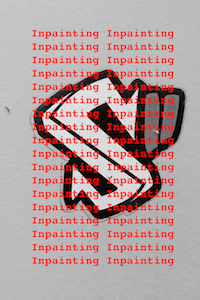
\includegraphics[width=4cm]{letter_pesc}}\hspace{0.2cm}
\subfigure[\label{fig:inpainting}]{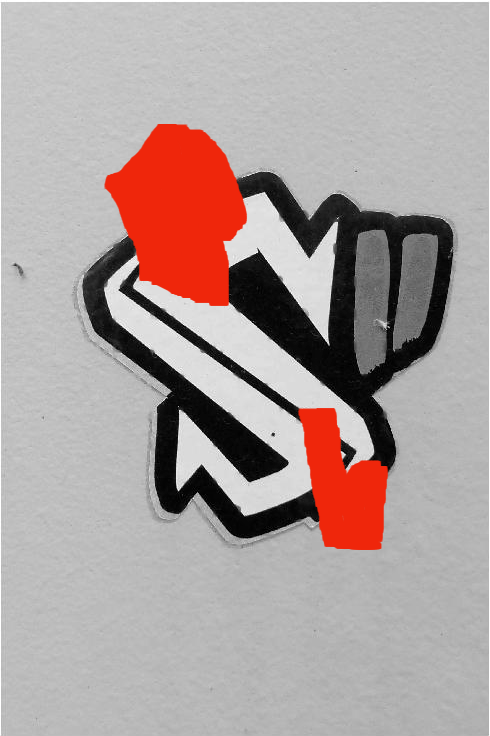
\includegraphics[width=4cm]{letter_inpainting}}
\caption{Different examples of inpainting domains, whereby the red parts are the inpainting domain.}
\end{center}
\end{figure}


\subsection{Impact and Continuation of the Project}


\paragraph{Supplements.}\todo{Here could go: nonconvex regularizer, different data terms, ...}
%We are going to consider additional topics for enriching the understanding of adaptive mechanisms by aspects that are different to the setting above. 


%In order to understand better the behavior of the $L^1$-$L^2$-TV model we intend to investigate its edge-preserving and scale-dependent properties for noise-free as well as for noisy data.
%
%We also want to extend the adaptive mechanisms to further applications, as the reconstruction from partial Fourier-data, which is a problem in magnetic resonance imaging, and wavelet inpainting, which is about restoring missing wavelet coefficients due to lossy compression or error-prone data transmission (see \cite{ChaSheZho, ZhaCha}). Note, that in these applications the observed data is not an image but frequencies and wavelet coefficients, respectively. Yet it is not clear at all how an adaptive meshing should be reasonable performed in such problems.
%
%Recently the $L^1$-$L^2$-TV model has been adapted to the $L^1$-$L^2$-TGV model in \cite{LiuShiYu Wan2015} by replacing the total variation term by the total generalized variation. Of course also other types of regularizers might be considered in this context, as the Mumford-Shah regularizer~\cite{GuMoNo}, higher-order regularizer, the nonlocal total variation and the $B_{1,1}^1$ Besov norm~\cite{Oswald:94, Triebel:78}. Note, that computing a minimizer using one of the aforementioned regularizers instead of the the total variation may improve the quality of the solution by the cost of increased computational complexity. Therefore it is indeed interesting to introduce %and in order to improve the restoration quality we want to introduce an 
%adaptive finite element methods for functionals consisting of a combined $L^1$/$L^2$ data fidelity term and one of the before mentioned regularizers.

\todo{Application medical imaging as a continuation project}

\subsection{Responsibilities of the investigators}


\subsubsection{Dr. Andreas Langer}

A. Langer is an expert in the field of mathematical image reconstruction, optimization and inverse problems. Hence he knows how to tackle the considered applications in an optimization framework and has experience in deriving and analysing locally adaptive parameter selection methods. Due to his expertise, he is responsible for 
\begin{enumerate}[(1)]
\item the development and analysis of the adaptive discretization techniques;
\item the development and analysis of the adaptive regularization methods;
\item the supervision of the postdoc researcher and doctoral student for the derivation of the adaptive methods, their numerical implementation, and their validation  
\end{enumerate} 
%development and analysis of the adaptive regularisation methods, their implementation and evaluation. % of the image reconstruction problems, finding corresponding convergent methods to obtain a solution, and the numerical implementation and evaluation. 



\subsubsection{Dr. Fernando Gaspoz}
F. Gaspoz has a strong background in functional analysis and is an expert for a posteriori estimates for adaptive finite elements. Hence in this project he is responsible for 
\begin{enumerate}[(1)]
\item  the derivation of the a posteriori estimates for the respective problems and the adaptive discretization approaches;
\item the supervision of the postdoc researcher and doctoral student for the derivation of the adaptive finite element methods and analytical aspects involved in the project;
\end{enumerate}

 
%\begin{enumerate}
%\item Consider clean images, as in [Bartels], [Hinterm\"uller, Rincon] for the $L^2$-TV model, now for the $L^1$-$L^2$-TV model and construct an adaptive finite element method. Is expected to work very similar as in previous work
%\item Noisy images, as in [Hinterm\"uller, Rincon] for the $L^2$-TV model, now for the $L^1$-$L^2$-TV model. May work similar but could be different since it should be able to treat a mixture of noise.
%\item Inpainting (+ noise): An adaptive FEM has not yet be considered for this application. 
%\item wavelet-inpainting (+ noise)
%\item reconstruction from partial Fourier-data (+ noise)
%\item Using different regularizers to improve restoration. For example consider Mumford-Shah regularizer for inpainting, Euler-Elastica model for inpainting, higher order regularizer for any application, nonlocal TV, TGV, ...
%\item Consider different algorithms (first and second order) and compare. For each algorithm one has to calculate aposteriori estimates separately.
%
%\item Find efficient solvers for the adaptive FE discretization, e.g., subspace correction methods.
%\end{enumerate}


% With this proposal we want to continue the successful
% work on the analysis of adaptive methods for \ppdes. 
%The research program described above has a rich and prosperous potential. 

% \subsection{Data handling}
% \label{sec:data-handling}
% Does not apply.

% \subsection{Other information}
% \label{sec:other-information}
% Does not apply.

% \subsection{Descriptions of proposed investigations involving experiments on humans, human materials or animals}
% \label{sec:proposed-investigations}
% Does not apply.


% \subsection{Information on scientific and financial involvement of international cooperation partners}
% \label{sec:cooperations}
% Does not apply.

%\small
\section{Bibliography}%
\makeatletter
\renewcommand{\@biblabel}[1]{[#1]}
\renewcommand*\bib@heading{%
%\subsection{Own Contributions}%
}
\makeatother
\iffalse
\bibliographystyle{acm}
% mbplain
\bibliography{nmh,para}
\else
%\small
\begin{thebibliography}{99}\itemsep=-3.5pt

\bibitem{AdaFou}
{\sc Adams, R. A. and Fournier, J. J. F.}
\newblock{\it Sobolev spaces}.
\newblock volume 140 of Pure and Applied Mathematics (Amsterdam). Elsevier/Academic Press, Amsterdam, second edition, 2003.

\bibitem{AinOde}
{\sc Ainsworth, M., and Oden, J.~T.}
\newblock {\em A Posteriori Error Estimation in Finite Element Analysis}.
\newblock Wiley-Interscience, New York, 2000.

%\bibitem{AlkLan}
%{\sc Alk\"amper, M. and Langer, A.}
%\newblock{Using DUNE-ACFem for non-smooth minimization of bounded variation functions}.
%\newblock{\em submitted to Archive of Numerical Software}, (2016), pp. 13.

\bibitem{All}
{\sc Alliney, S.}
\newblock{A property of the minimum vectors of a regularizing functional defined by means of the absolute norm}.
\newblock{\em IEEE Transactions on Signal Processing 45}, 4 (1997), 913--917.
 
\bibitem{AmbFusPal}
{\sc Ambrosio, L., Fusco, N., and Pallara, D.}
\newblock{\it Functions of bounded variation and free discontinuity problems}.
\newblock Oxford Mathematical Monographs. The Clarendon Press, Oxford University Press, New York, 2000.

\bibitem{BanJos} 
{\sc Bangerth, W., and Joshi, A.}
\newblock {Adaptive finite element methods for the solution of inverse problems in optical tomography}.
\newblock {\em Inverse Problems 24}, 3 (2008), pp 22.

\bibitem{BanRan}
{\sc Bangerth, W., and Rannacher, R.}
\newblock {\em Adaptive Finite Element Methods for Differential Equations}.
\newblock Lectures in Mathematics, ETH Z\"urich. Birkh\"auser, Basel, 2003.

\bibitem{BazBlo} 
{\sc Bazan, C and Blomgren, P.}
\newblock {Adaptive finite element method for image processing}.
\newblock {\em Report - Publication number: CSRCR2006-15}, (2006), pp 6.

\bibitem{Bar2012} 
{\sc Bartels, S.}
\newblock {Total variation minimization with finite elements: convergence and iterative solution}.
\newblock {\em SIAM J. Numer. Anal. 50}, 3 (2012), 1162--1180.

\bibitem{Bar2013} 
{\sc Bartels, S.}
\newblock {Broken Sobolev space iteration for total variation regularized minimization problems}.
\newblock {\em IMA Journal of Numerical Analysis}, (2015), pp. 10.

\bibitem{Bar2015} 
{\sc Bartels, S.}
\newblock {Error control and adaptivity for a variational model problem defined on functions of bounded variation}.
\newblock {\em Mathematics of Computation 84}, 293 (2015), 1217--1240.

\bibitem{BarNocSal} 
{\sc Bartels, S., Nochetto, R. H., and Salgado, A. J. }
\newblock {Discrete total variation flows without reglarization}.
\newblock {\em SIAM J. Numer. Anal. 52}, 1 (2014), 363--385.

\bibitem{BaeMik}
{\sc B\"ansch, e. and Mikula, K.}
\newblock{A coarsening finite element strategy in image selective smoothing}.
\newblock{\em Computing and Visualization in Science 1}, (1997), 53--61.

\bibitem{Bov}
{\sc Bovik, A.}
\newblock{\it Handbook of Image and Video Processing}.
\newblock Academic Press, San Diego, 2000.

\bibitem{BreKunPoc}
{\sc Bredies, K. and Kunisch, K. and Pock, T.}
\newblock{Total generalized variation}.
\newblock{\em SIAM Journal on Imaging Sciences 3}, 3 (2010), 492--526.

\bibitem{Car}
{\sc Carey, G.~F.}
\newblock {\em Computational Grids: Generation, Adaptation and Solution Strategies}.
\newblock Taylor and Francis, London, 1997.

\bibitem{CatLioMorCol}
{\sc Catt\'e, F., Lion, P. L., Morel, J. M., and Coll, T.}
\newblock{Image selective smoothing and edge detection by nonlinear diffusion}.
\newblock{\em SIAM Journal Numer. Anal. 129}, (1992), 182--193.

\bibitem{Cha}
{\sc Chambolle, A.} 
\newblock{An algorithm for total variation minimization and applications}. 
\newblock{\em J. Math. Imaging Vision 20}, 1-2 (2004), 89--97.

\bibitem{ChaDar}
{\sc Chambolle, A. and Darbon, J.} 
\newblock{On total variation minimization and surface evolution using parametric maximum flows}. \newblock{\em International journal of computer vision 84}, 3 (2009), 288--307.

\bibitem{ChaLio}
{\sc Chambolle, A. and Lions,P.-L.}
\newblock{ Image recovery via total variation minimization and related problems}. 
\newblock{\em Numer. Math. 76}, 2 (1997), 167--188.

\bibitem{ChaPoc}
{\sc Chambolle, A. and Pock, T.} 
\newblock{A first-order primal-dual algorithm for convex problems with applications to imaging}. 
\newblock{\em J. Math. Imaging Vision 40}, 1 (2011), 120--145.

\bibitem{ChaHoNik}
{\sc Chan, R. H. and Ho, Ch.-W. and Nikolova, M.}
\newblock{Salt-and-pepper noise removal by median-type noise detectors and detail-preserving regularization},
\newblock{\em IEEE Transactions on Image Processing 14}, 10 (2005), 1479--1485

\bibitem{ChaGolMul}
{\sc Chan, T. F., Golub, G. H., and Mulet P.}
\newblock{ A nonlinear primal-dual method for total variation-based image restoration}. 
\newblock{\em SIAM J. Sci. Comput. 20}, 6 (1999), 1964--1977.

\bibitem{ChaKanShe}
{\sc Chan, T. F., Kang, S. H., and Shen J.}
\newblock{ Euler's Elastica and curvature-based inpainting}. 
\newblock{\em SIAM J. Appl. Math. 63}, 2 (2002), 564--592.

\bibitem{ChaSheZho}
{\sc Chan, T. F., Shen, J., and Zhou, H.-M.}
\newblock{Total variation wavelet inpainting}. 
\newblock{\em J. Math. Imaging Vision 1}, 25 (2006), 107--125.

\bibitem{Ciarlet:02}
{\sc Ciarlet, P.~G.}
\newblock {\em The finite element method for elliptic problems}, vol.~40 of  {\em Classics in Applied Mathematics}.
\newblock Society for Industrial and Applied Mathematics (SIAM), Philadelphia, PA, 2002.

\bibitem{ComWaj}
{\sc Combettes, P. L. and Wajs, V. R.} 
\newblock{Signal recovery by proximal forward-backward splitting}.
\newblock{\em Multiscale Model. Simul. 4}, 4 (2005), 1168--1200.

\bibitem{DarSig05}
{\sc Darbon, J. and Sigelle, M.}
\newblock{ A fast and exact algorithm for total variation minimization}.
\newblock{\em In Pattern recognition and image analysis}, Springer (2005), 351--359.

\bibitem{DarSig06}
{\sc Darbon, J. and Sigelle, M.}
\newblock{ Image restoration with discrete constrained total variation. I. Fast and exact optimization.}
\newblock{ \em  J. Math. Imaging Vision 26}, 3 (2006), 261--276.

\bibitem{DauTesVes}
{\sc Daubechies, I., Teschke, G., and Vese, L.} 
\newblock{Iteratively solving linear inverse problems under general convex constraints.} 
\newblock{\em Inverse Probl. Imaging 1}, 1 (2007), 29--46.

\bibitem{DesJaoSel}
{\sc Destuynder, Ph., Jaoua, M., and Sellami, H.}
\newblock{An error estimate in image processing.} 
\newblock{ \em ARIMA Journal 15}, (2012), 61--81.

\bibitem{DobVog}
{\sc Dobson, D. C. and Vogel, C. R.}
\newblock{ Convergence of an iterative method for total variation denoising.} 
\newblock{ \em SIAM J. Numer. Anal. 34} 5 (1997), 1779--1791.

\bibitem{EngHanNeu}
{\sc Engl, H. W., Hanke, M., and Neubauer, A.}
\newblock{\it Regularization of inverse problems}.
\newblock Mathematics and its Applications. Kluwer Academic Publishers Group, Dordrecht, 1996.

\bibitem{GabMer}
{\sc Gabay, D. and Mercier, B.}
\newblock{ A dual algorithm for the solution of nonlinear variational problems via finite-element approximations.} 
\newblock{ \em Comput. Optim. Appl. 2} (1976), 17--40.

\bibitem{Giu}
{\sc Giusti, E.}
\newblock{\it Minimal surfaces and functions of bounded variation}
\newblock volume 80 of Monographs in Mathematics. Birkh\"auser Verlag, Basel, 1984

\bibitem{Glo}
{\sc Glowinski, R.}
\newblock{\it Numerical Methods for Nonlinear Variational Problems}.
\newblock Springer-Verlag, New York, 1984.

\bibitem{GolOsh}
{\sc Goldstein, T. and Osher, S.} 
\newblock{The split Bregman method for $L^1$-regularized problems.} 
\newblock{\em SIAM J. Imaging Sci. 2} 2 (2009), 323--343.

\bibitem{GonSheToh2014} 
{\sc Gong, Z., Shen, Z., and Toh, K.-C.}
\newblock {Image restoration with mixed or unknown noises}.
\newblock {\em Multiscale Model. Simul. 12}, 2 (2014), 458--487.

\bibitem{GuMoNo}
{\sc Do{\v{g}}an, G. , Morin, P. and Nochetto, R. H.} 
\newblock{A variational shape optimization approach for image
              segmentation with a {M}umford-{S}hah functional.} 
\newblock{\em SIAM J. Sci. Comput. 30} 6 (2008), 3028--3049.

%\bibitem{HinLan2013} 
%{\sc Hinterm\"uller, M., and Langer, A.}
%\newblock {Subspace correction methods for a class of nonsmooth and nonadditive convex variational problems with mixed $L^1/L^2$ data-fidelity in image processing}.
%\newblock {\em SIAM J. Imaging Sciences 6}, 4 (2013), 2134--2173.

\bibitem{HinRin2014} 
{\sc Hinterm\"uller, M., and Rincon-Camacho, M.}
\newblock {An adaptive finite element method in $L^2$-TV-based image denoising}.
\newblock {\em Inverse Problems and Imaging 8}, 3 (2014), 685--711.

\bibitem{HinSta}
{\sc Hinterm\"uller, M. and Stadler, G.}
\newblock{ An infeasible primal-dual algorithm for total bounded variation-based inf-convolution-type image restoration.}
\newblock{SIAM J. Sci. Comput. 28}, 1 (2006), 1--23.

\bibitem{KinOshJon}
{\sc Kindermann, S., Osher, S., and Jones, P. W. }
\newblock{Deblurring and denoising of images by nonlocal functionals}.
\newblock {\em Multiscale Model. Simul. 4}, 4 (2005), 1091--1115

\bibitem{KoRoSi:14}
 {\sc Kohls, K.,  R\"osch, A. and  Siebert, K.\,G.}
\newblock A Posteriori error analysis of optimal control problems with control constraints.
\newblock {\em SIAM J. Control Optim.}, 52(3):1832--1861, 2014.

\bibitem{Lam}
{\sc Lamichhane, B.}
\newblock {Finite element techniques for removing the mixture of Gaussian and impulsive noise}.
\newblock {\em IEEE Transactions on Signal Processing 57}, 7 (2009), 2538--2547.

\bibitem{Lan2015} 
{\sc Langer A.}
\newblock {Automated parameter selection for total variation minimization in image restoration}.
\newblock { {\em J. Math. Imaging Vis.}}, (2016), pp. 30.

%\bibitem{Lan2016} 
%{\sc Langer A.}
%\newblock {Automated parameter selection in the $L^1$-$L^2$-TV model for removing Gaussian plus impulse noise}.
%\newblock { submitted to {\em Inverse Problems}}, (2016), pp. 29.

\bibitem{Li} 
{\sc Li, J.}
\newblock{Finite element analysis for a nonlinear diffusion model in image processing}.
\newblock {\em Applied Mathematics Letter 15}, (2002), 197--202.

\bibitem{LiuShiYu Wan2015} 
{\sc Liu, R. W., Shi, L., Yu, S. C. H., and Wang, D.}
\newblock {Box-constrained second-order total generalized variation minimization with a combined $L^{1,2}$ data-fidelity term for image reconstruction}.
\newblock {\em Journal of Electronic Imaging 24}, 3 (2015), 033026--033026.

\bibitem{Lov}
{\sc Love, A. E. H.}
\newblock{\it A Treatise on the Mathematial Theory of Elasticity},
\newblock Dover, 4th ed., 1927.

\bibitem{Moe}
{\sc Moeslund, T. B.}
\newblock{\it Introduction to video and image processing: Building real systems and applications},
\newblock Springer Science \& Business Media, 2012

\bibitem{Nes}
{\sc Nesterov, Y.}
\newblock{Smooth minimization of non-smooth functions.}
\newblock{\em  Math. Program. 103} 1, Ser. A (2005), 127--152.

\bibitem{Nik2002}
{\sc Nikolova, M.}
\newblock{Minimizers of cost-functions involving nonsmooth data-fidelity
              terms. {A}pplication to the processing of outliers}.
 \newblock{\em SIAM Journal on Numerical Analysis 40}, 3 (2002), 965--994.

\bibitem{Nik2004}
{\sc Nikolova, M.}
\newblock{A variational approach to remove outliers and impulse noise}.
 \newblock{\em Journal of Mathematical Imaging and Vision 20}, 1-2 (2004), 99--120.
 
\bibitem{NoSiVe:09}
{\sc Nochetto, R.~H., Siebert, K.~G., and Veeser, A.}
\newblock Theory of adaptive finite element methods: an introduction.
\newblock In {\em Multiscale, nonlinear and adaptive approximation}. Springer, Berlin, 2009, pp.~409--542.


\bibitem{OshBurGolXuYin}
{\sc Osher, S., Burger, M., Goldfarb, D., Xu, J., and Yin, W.}
\newblock{ An iterative regularization method for total variation-based image restoration.} 
\newblock{\em Multiscale Model. Simul. 4}, 2 (2005), 460--489.

\bibitem{Oswald:94}
{\sc Oswald, P.}
\newblock {\em Multilevel finite element approximation: Theory and applications}.
\newblock Teubner Skripten zur Numerik. B. G. Teubner, Stuttgart, 1994.

\bibitem{PapSch}
{\sc Papafitsoros, K. and Sch\"onlieb, C. B.}
\newblock{A combined first and second order variationsl approach for image reconstruction}.
\newblock{\em Journal of mathematical imaging and vision 48}, 2 (2014), 308--338.

\bibitem{PerMal}
{\sc Perona, P. and Malik, J. }
\newblock{Scale-space and edge detection using anisotropic diffusion.}
\newblock{\em IEEE Transactions on Pattern Analysis and Machine Intelligence 12}, 7 (1990), 629--639.


\bibitem{PreRum}
{\sc Preu\ss er, T. and Rumpf, M. }
\newblock{An adaptive finite element method for large scale image processing}.
\newblock{\em Journal of Visual Communication and Image Representation 11}, (2000), 183--195.


\bibitem{Repin} 
{\sc Repin, S. I.}
\newblock{A posteriori error estimation for variational problems with
              uniformly convex functionals}.
\newblock{Math. Comp.  69},230 (2000), 481--500.

\bibitem{ROF} 
{\sc Rudin, L. I., Osher, S., and Fatemi, E.}
\newblock{Nonlinear total variation based noise removal algorithms}.
\newblock{Physica D: Nonlinear Phenomena 60},1 (1992), 259--268.

\bibitem{Verfurth:96}
{\sc Verf\"urth, R.}
\newblock {\em A Review of A Posteriori Error Estimation and Adaptive  Mesh-Refinement Techniques}.
\newblock Adv. Numer. Math. John Wiley, Chichester, UK, 1996.

\bibitem{TiaYua}
{\sc Tian, W. Y. and Yuan, X.}
\newblock{ Convergence analysis of primal-dual based methods for total variation minimization with finite element approximation.}
\newblock{\em preprint}, (2015), pp. 27.

\bibitem{Triebel:78}
{\sc Triebel, H.}
\newblock {\em Interpolation theory, function spaces, differential operators}.
\newblock North-Holland Mathematical Library, 18. North-Holland Publishing Co., Amsterdam-New York, 1978.


\bibitem{WeiBlaAub}
{\sc Weiss, P., Blanc-Feraud, L., and Aubert, G.}
\newblock{ Efficient schemes for total variation minimization under constraints in image processing.}
\newblock{\em SIAM J. Sci. Comput. 31}, 3 (2009), 2047--2080.

\bibitem{Yao}
{\sc Yao, C. H.}
\newblock{Finite element approximation for {TV} regularization.}
\newblock{\em International Journal of Numerical Analysis and Modeling 5}, 3 (2008), 516--526.

\bibitem{ZhaCha}
{\sc Zhang, X. and Chan, T. F.}
\newblock{Wavelet inpainting by nonlocal total variation.}
\newblock{\em Inverse Problems and Imaging 4}, 1 (2010), 191--210.

%\bibitem{AinsworthOden:00}
%{\sc Ainsworth, M., and Oden, J.~T.}
%\newblock {\em A Posteriori Error Estimation in Finite Element Analysis}.
%\newblock Wiley-Interscience, New York, 2000.
%
%\bibitem{BabuskaMakridakis:97}
%{\sc Babu{\v{s}}ka, I., and Makridakis, C.}
%\newblock On the stability of the discontinuous {G}alerkin method for the heat
%  equation.
%\newblock {\em SIAM J. Numer. Anal. 34\/} (1997), 389--401.
%
%\bibitem{BabuskaStrouboulis:01}
%{\sc Babu{\v{s}}ka, I., and Strouboulis, T.}
%\newblock {\em The finite element method and its reliability}.
%\newblock Numerical Mathematics and Scientific Computation. The Clarendon Press
%  Oxford University Press, 2001.
%
%\bibitem{Babuska:71}
%{\sc Babu\v{s}ka, I.}
%\newblock Error-bounds for finite element method.
%\newblock {\em Numer. Math. 16\/} (1971), 322--333.
%
%\bibitem{BaiocchiBrezzi:83}
%{\sc Baiocchi, C., and Brezzi, F.}
%\newblock Optimal error estimates for linear parabolic problems under minimal
%  regularity assumptions.
%\newblock {\em Calcolo 20}, 2 (1983), 143--176.
%
%\bibitem{BangerthRannacher:03}
%{\sc Bangerth, W., and Rannacher, R.}
%\newblock {\em Adaptive Finite Element Methods for Differential Equations}.
%\newblock Lectures in Mathematics, ETH Z\"urich. Birkh\"auser, Basel, 2003.
%
%\bibitem{BankSantos:93}
%{\sc Bank, R.~E., and Santos, R.~F.}
%\newblock Analysis of some moving space-time finite element methods.
%\newblock {\em SIAM J. Numer. Anal. 30}, 1 (1993), 1--18.
%
%\bibitem{BankYserentant:14}
%{\sc Bank, R.~E., and Yserentant, H.}
%\newblock On the {$H^1$}-stability of the {$L_2$}-projection onto finite
%  element spaces.
%\newblock {\em Numerische Mathematik 126}, 2 (2014), 361--381.
%
%\bibitem{BaKaMa:13}
%{\sc B{\"a}nsch, E., Karakatsani, F., and Makridakis, C.}
%\newblock The effect of mesh modification in time on the error control of fully
%  discrete approximations for parabolic equations.
%\newblock {\em Appl. Numer. Math. 67\/} (2013), 35--63.
%
%\bibitem{BaMoNo:02}
%{\sc B{\"a}nsch, E., Morin, P., and Nochetto, R.~H.}
%\newblock An adaptive {U}zawa {FEM} for the {S}tokes problem: convergence
%  without the inf-sup condition.
%\newblock {\em SIAM J. Numer. Anal. 40}, 4 (2002), 1207--1229.
%
%\bibitem{dune:06}
%{\sc Bastian, P., Blatt, M., Dedner, A., Engwer, C., Kl\"ofkorn, R.,
%  Kuttanikkad, S., {Ohl\-ber\-ger}, M., and Sander, O.}
%\newblock {The Distributed and Unified Numerics Environment (DUNE)}.
%\newblock In {\em Proc. of the 19th Symposium on Simulation Technique in
%  Hannover, Sep. 12 - 14\/} (2006).
%
%\bibitem{BeckerMao:11b}
%{\sc Becker, R., and Mao, S.}
%\newblock Quasi-optimality of adaptive nonconforming finite element methods for
%  the {S}tokes equations.
%\newblock {\em SIAM J. Numer. Anal. 49}, 3 (2011), 970--991.
%
%\bibitem{BeckerMao:11a}
%{\sc Becker, R., and Mao, S.}
%\newblock Quasi-optimality of an adaptive finite element method for an optimal
%  control problem.
%\newblock {\em Comput. Methods Appl. Math. 11}, 2 (2011), 107--128.
%
%\bibitem{BeRa:96}
%{\sc Becker, R., and Rannacher, R.}
%\newblock Weighted a posteriori error control in {FE} methods.
%\newblock {\em Lecture ENUMATH-95\/} (1996).
%
%\bibitem{BeckerRannacher:01}
%{\sc Becker, R., and Rannacher, R.}
%\newblock An optimal control approach to a posteriori error estimation in
%  finite element methods.
%\newblock {\em Acta Numer. 10\/} (2001), 1--102.
%
%\bibitem{BeDiKr:12}
%{\sc Belenki, L., Diening, L., and Kreuzer, C.}
%\newblock Optimality of an adaptive finite element method for the
%  $p$-{L}aplacian equation.
%\newblock {\em IMA J. of Numer. Anal. 32}, 2 (2012), 484--510.
%
%\bibitem{BernardiHechtVerfurth:09}
%{\sc Bernardi, C., Hecht, F., and Verf{\"u}rth, R.}
%\newblock A finite element discretization of the three-dimensional
%  {N}avier-{S}tokes equations with mixed boundary conditions.
%\newblock {\em M2AN Math. Model. Numer. Anal. 43}, 6 (2009), 1185--1201.
%
%\bibitem{Berrone:06}
%{\sc Berrone, S.}
%\newblock Robust a posteriori error estimates for finite element
%  discretizations of the heat equation with discontinuous coefficients.
%\newblock {\em M2AN Math. Model. Numer. Anal. 40}, 6 (2006), 991--1021.
%
%\bibitem{BiDaDe:04}
%{\sc Binev, P., Dahmen, W., and DeVore, R.}
%\newblock Adaptive finite element methods with convergence rates.
%\newblock {\em Numer. Math 97\/} (2004), 219--268.
%
%\bibitem{BiDaDePe:02}
%{\sc Binev, P., Dahmen, W., DeVore, R., and Petrushev, P.}
%\newblock Approximation classes for adaptive methods.
%\newblock {\em Serdica Math. J. 28}, 4 (2002), 391--416.
%\newblock Dedicated to the memory of Vassil Popov on the occasion of his 60th
%  birthday.
%
%\bibitem{BinevDeVore:04}
%{\sc Binev, P., and DeVore, R.}
%\newblock Fast computation in adaptive tree approximation.
%\newblock {\em Numer. Math. 97}, 2 (2004), 193--217.
%
%\bibitem{BonitoNochetto:10}
%{\sc Bonito, A., and Nochetto, R.~H.}
%\newblock Quasi-optimal convergence rate of an adaptive discontinuous
%  {G}alerkin method.
%\newblock {\em SIAM J. Numer. Anal. 48}, 2 (2010), 734--771.
%
%\bibitem{Braess:13}
%{\sc Braess, D.}
%\newblock {\em Finite Elemente: Theorie, schnelle {L\"o}ser und {A}nwendungen
%  in der {E}lastizit{\"a}tstheorie}, 5. {\"u}berarb. aufl.~ed.
%\newblock Springer Spektrum, Berlin, 2013.
%
%\bibitem{BrCaHo:07}
%{\sc Braess, D., Carstensen, C., and Hoppe, R. H.~W.}
%\newblock Convergence analysis of a conforming adaptive finite element method
%  for an obstacle problem.
%\newblock {\em Numer. Math. 107}, 3 (2007), 455--471.
%
%\bibitem{BrPaSt:02}
%{\sc Bramble, J.~H., Pasciak, J.~E., and Steinbach, O.}
%\newblock On the stability of the ${L^2}$ projection in ${H^1(\Omega)}$.
%\newblock {\em Math. Comput. 71}, 237 (2002), 147--156.
%
%\bibitem{BrennerScott:08}
%{\sc Brenner, S.~C., and Scott, L.~R.}
%\newblock {\em The mathematical theory of finite element methods}, third~ed.,
%  vol.~15 of {\em Texts in Applied Mathematics}.
%\newblock Springer, New York, 2008.
%
%\bibitem{bddko:06}
%{\sc Burri, A., Dedner, A., Diehl, D., Kl\"ofkorn, R., and Ohlberger, M.}
%\newblock A general object oriented framework for discretizing non-linear
%  evolution equations.
%\newblock In {\em Advances in High Performance Computing and Computational
%  Sciences}, Y.~S. et~al., Ed., vol.~93. Springer, 2006, pp.~69--87.
%
%\bibitem{CaGeMe:13}
%{\sc Cangiani, A., Georgoulis, E.~H., and Metcalfe, S.}
%\newblock Adaptive discontinuous Galerkin methods for nonstationary convection/diffusion
%	problems. {\em IMA J. of Numer. Anal.}
%  51 (2013), 2911--2934.
%
%\bibitem{Carstensen:02}
%{\sc Carstensen, C.}
%\newblock Merging the {B}ramble-{P}asciak-{S}teinbach and the
%  {C}rouzeix-{T}hom\'ee criterion for {$H^1$}-stability of the
%  {$L^2$}-projection onto finite element spaces.
%\newblock {\em Math. Comp. 71}, 237 (2002), 157--163.
%
%\bibitem{Carstensen:04}
%{\sc Carstensen, C.}
%\newblock An adaptive mesh-refining algorithm allowing for an {$H^1$} stable
%  {$L^2$} projection onto {C}ourant finite element spaces.
%\newblock {\em Constr. Approx. 20}, 4 (2004), 549--564.
%
%\bibitem{CarstensenHoppe:05}
%{\sc Carstensen, C., and Hoppe, R. H.~W.}
%\newblock Convergence analysis of an adaptive edge finite element method for
%  the {2D} eddy current equations.
%\newblock {\em J. Numer. Math. 13}, 1 (2005), 19--32.
%
%\bibitem{CarstensenHoppe:06}
%{\sc Carstensen, C., and Hoppe, R. H.~W.}
%\newblock Error reduction and convergence for an adaptive mixed finite element
%  method.
%\newblock {\em Math. Comp. 75}, 255 (2006), 1033--1042.
%
%\bibitem{CaKrNoSi:08}
%{\sc Cascon, J.~M., Kreuzer, C., Nochetto, R.~H., and Siebert, K.~G.}
%\newblock Quasi-optimal convergence rate for an adaptive finite element method.
%\newblock {\em SIAM J. Numer. Anal. 46}, 5 (2008), 2524--2550.
%
%\bibitem{CasconNochetto:12}
%{\sc Casc{\'o}n, J.~M., and Nochetto, R.~H.}
%\newblock Quasioptimal cardinality of {AFEM} driven by nonresidual estimators.
%\newblock {\em IMA J. Numer. Anal. 32}, 1 (2012), 1--29.
%
%\bibitem{CaNoSi:07}
%{\sc Casc\'on, J.~M., Nochetto, R.~H., and Siebert, K.~G.}
%\newblock Design and convergence of {AFEM} in {H}({\rm div}).
%\newblock {\em Math. Models Methods Appl. 17\/} (2007), 1849--1881.
%
%\bibitem{Cea:64}
%{\sc Cea, J.}
%\newblock Approximation variationnelle des probl{\`e}mes aux limites.
%\newblock {\em Ann. Inst. Fourier 14}, 2 (1964), 345--444.
%
%\bibitem{ChXuHo:10}
%{\sc Chen, H., Xu, X., and Hoppe, R. H.~W.}
%\newblock Convergence and quasi-optimality of adaptive nonconforming finite
%  element methods for some nonsymmetric and indefinite problems.
%\newblock {\em Numer. Math. 116}, 3 (2010), 383--419.
%
%\bibitem{ChHoXu:09}
%{\sc Chen, L., Holst, M., and Xu, J.}
%\newblock Convergence and optimality of adaptive mixed finite element methods.
%\newblock {\em Math. Comp. 78}, 265 (2009), 35--53.
%
%\bibitem{ChenFeng:04}
%{\sc Chen, Z., and Feng, J.}
%\newblock An adaptive finite element algorithm with reliable and efficient
%  error control for linear parabolic problems.
%\newblock {\em Math. Comp. 73\/} (2004), 1167--1193.
%

%
%\bibitem{CoDaDe:02}
%{\sc Cohen, A., Dahmen, W., and DeVore, R.}
%\newblock Adaptive wavelet methods. {II}. {B}eyond the elliptic case.
%\newblock {\em Found. Comput. Math. 2}, 3 (2002), 203--245.
%
%\bibitem{DautrayLions:92}
%{\sc Dautray, R., and Lions, J.-L.}
%\newblock {\em Mathematical analysis and numerical methods for science and
%  technology. {V}ol. 5}.
%\newblock Springer-Verlag, Berlin, 1992.
%\newblock Evolution problems. I, With the collaboration of Michel Artola,
%  Michel Cessenat and H{\'e}l{\`e}ne Lanchon, Translated from the French by
%  Alan Craig.
%
%\bibitem{DebrabantLang:13}
%{\sc Debrabant, K., and Lang, J.}
%\newblock On global error estimation and control of finite difference solutions
%  for parabolic equations.
%\newblock In {\em VI International Conference on Adaptive Modeling and
%  Simulation {ADMOS} 2013\/} (2013), J.~P.~M. de~Almeida, P.~Diez, C.~Tiago,
%  and N.~Par\'es, Eds., Center for Numerical Methods in Engineering {(CIMNE)},
%  Barcelona, Spain, pp.~187--198.
%
%\bibitem{DeLaMa:09}
%{\sc Demlow, A., Lakkis, O., and Makridakis, C.}
%\newblock A posteriori error estimates in the maximun norm for parabolic
%  problems.
%\newblock {\em SIAM J. Numer. Anal. 47}, 3 (2009), 2157--2176.
%
%\bibitem{DemStev:11}
%{\sc Demlow, A., and Stevenson, R.}
%\newblock Convergence and quasi-optimality of an adaptive finite element method
%  for controlling {$L_2$} errors.
%\newblock {\em Numer. Math. 117}, 2 (2011), 185--218.
%
%\bibitem{DieningKreuzer:08}
%{\sc Diening, L., and Kreuzer, C.}
%\newblock Convergence of an adaptive finite element method for the
%  $p$-{L}aplacian equation.
%\newblock {\em SIAM J. Numer. Anal. 46}, 2 (2008), 614--638.
%
%\bibitem{DiKrSt:13}
%{\sc Diening, L., Kreuzer, C., and Stevenson, R.}
%\newblock Instance optimality of the adaptive maximum strategy.
%\newblock {\em Preprint-Arxiv\/} (2013).
%
%\bibitem{Dorfler:96}
%{\sc D{\"o}rfler, W.}
%\newblock A convergent adaptive algorithm for {P}oisson's equation.
%\newblock {\em SIAM J. Numer. Anal. 33}, 3 (1996), 1106--1124.
%
%\bibitem{DouglasDupont:70}
%{\sc Douglas, Jr., J., and Dupont, T.}
%\newblock Galerkin methods for parabolic equations.
%\newblock {\em SIAM J. Numer. Anal. 7\/} (1970), 575--626.
%
%\bibitem{DuXie:12}
%{\sc Du, S., and Xie, X.}
%\newblock Error reduction, convergence and optimality of an adaptive mixed
%  finite element method.
%\newblock {\em J. Syst. Sci. Complex. 25}, 1 (2012), 195--208.
%
%\bibitem{Dupont:82}
%{\sc Dupont, T.}
%\newblock Mesh modification for evolution equations.
%\newblock {\em Math. Comp. 39}, 159 (1982), 85--107.
%
%\bibitem{ErikssonJohnson:91}
%{\sc Eriksson, K., and Johnson, C.}
%\newblock Adaptive finite element methods for parabolic problems {I}: {A}
%  linear model problem.
%\newblock {\em SIAM J. Numer. Anal. 28\/} (1991), 43--77.
%
%\bibitem{ErikssonJohnson:95a}
%{\sc Eriksson, K., and Johnson, C.}
%\newblock Adaptive finite element methods for parabolic problems. {IV}.
%  {N}onlinear problems.
%\newblock {\em SIAM J. Numer. Anal. 32}, 6 (1995), 1729--1749.
%
%\bibitem{ErikssonJohnson:95b}
%{\sc Eriksson, K., and Johnson, C.}
%\newblock Adaptive finite element methods for parabolic problems. {V}.
%  {L}ong-time integration.
%\newblock {\em SIAM J. Numer. Anal. 32}, 6 (1995), 1750--1763.
%
%\bibitem{FeFuPr:14}
%{\sc Feischl, M., F{\"u}hrer, T., and Praetorius, D.}
%\newblock Adaptive {FEM} with optimal convergence rates for a certain class of
%  nonsymmetric and possibly nonlinear problems.
%\newblock {\em SIAM J. Numer. Anal. 52}, 2 (2014), 601--625.
%
%\bibitem{GarauMorin:11}
%{\sc Garau, E.~M., and Morin, P.}
%\newblock Convergence and quasi-optimality of adaptive {FEM} for {S}teklov
%  eigenvalue problems.
%\newblock {\em IMA J. Numer. Anal. 31}, 3 (2011), 914--946.
%
%\bibitem{GaMoZu:12}
%{\sc Garau, E.~M., Morin, P., and Zuppa, C.}
%\newblock Quasi-optimal convergence rate of an {AFEM} for quasi-linear problems
%  of monotone type.
%\newblock {\em Numer. Math. Theory Methods Appl. 5}, 2 (2012), 131--156.
%
%\bibitem{GaspozMorin:09}
%{\sc Gaspoz, F.~D., and Morin, P.}
%\newblock Convergence rates for adaptive finite elements.
%\newblock {\em IMA J. Numer. Anal. 29}, 4 (2009), 917--936.
%
%\bibitem{GeLaVi:11}
%{\sc Georgoulis, E.~H., Lakkis, O., and Virtanen, J.~M.}
%\newblock A posteriori error control for discontinuous galerkin methods for
%  parabolic problems.
%\newblock {\em SIAM J. Numer. Anal. 49}, 2 (2011), 427--458.
%
%\bibitem{HuangXu:12}
%{\sc Huang, J., and Xu, Y.}
%\newblock Convergence and complexity of arbitrary order adaptive mixed element
%  methods for the {P}oisson equation.
%\newblock {\em Sci. China Math. 55}, 5 (2012), 1083--1098.
%
%\bibitem{KaPaPr:13}
%{\sc Karkulik, M., Pavlicek, D., and Praetorius, D.}
%\newblock On 2{D} newest vertex bisection: optimality of mesh-closure and
%  {$H^1$}-stability of {$L_2$}-projection.
%\newblock {\em Constr. Approx. 38}, 2 (2013), 213--234.
%
%\bibitem{Kohls:13}
%{\sc Kohls, K.}
%\newblock {\em An Adaptive Finite Element Method for Control-Constrained
%  Optimal Control Problems}.
%\newblock PhD thesis, Fachbereich Mathematik, Unversit\"at Stuttgart, 2013.
%
%\bibitem{KoRoSi:12}
%{\sc Kohls, K., R{\"o}sch, A., and Siebert, K.~G.}
%\newblock A posteriori error estimators for control constrained optimal control
%  problems.
%\newblock In {\em Constrained optimization and optimal control for partial
%  differential equations}, vol.~160 of {\em Internat. Ser. Numer. Math.}
%  Birkh\"auser/Springer Basel AG, Basel, 2012, pp.~431--443.
%
%\bibitem{KoRoSi:13a}
%{\sc Kohls, K., R{\"o}sch, A., and Siebert, K.~G.}
%\newblock Convergence of adaptive finite elements for control constrained
%  optimal control problems.
%\newblock Stuttgarter Mathematische Berichte 2013-011, Preprint SPP1253-153, 2013.
%
%\bibitem{LaMa:06}
%{\sc Lakkis, O., and Makridakis, C.}
%\newblock Elliptic reconstruction and a posteriori error estimates for fully
%  discrete linear parabolic problems.
%\newblock {\em Math. Comp. 75}, 256 (2006), 1627--1658.
%
%\bibitem{MakridakisNochetto:03}
%{\sc Makridakis, C., and Nochetto, R.~H.}
%\newblock Elliptic reconstruction and a posteriori error estimates for
%  parabolic problems.
%\newblock {\em SIAM J. Numer. Anal. 41}, 4 (2003), 1585--1594.
%
%\bibitem{MeidnerVexler:07}
%{\sc Meidner, D., and Vexler, B.}
%\newblock Adaptive space-time finite element methods for parabolic optimization
%  problems.
%\newblock {\em SIAM J. Control Optim. 46}, 1 (2007), 116--142.
%
%\bibitem{Moeller:10b}
%{\sc M\"oller, C.~A.}
%\newblock {\em Adaptive Finite Elements in the Discretization of Parabolic
%  Problems}.
%\newblock PhD thesis, Universit\"at Augsburg, 2010.
%
%\bibitem{MommerStevenson:09}
%{\sc Mommer, M.~S., and Stevenson, R.}
%\newblock A goal-oriented adaptive finite element method with convergence
%  rates.
%\newblock {\em SIAM J. Numer. Anal. 47}, 2 (2009), 861--886.
%
%\bibitem{MoNoSi:00}
%{\sc Morin, P., Nochetto, R.~H., and Siebert, K.~G.}
%\newblock Data oscillation and convergence of adaptive {FEM}.
%\newblock {\em SIAM J. Numer. Anal. 38\/} (2000), 466--488.
%
%\bibitem{MoNoSi:02}
%{\sc Morin, P., Nochetto, R.~H., and Siebert, K.~G.}
%\newblock Convergence of adaptive finite element methods.
%\newblock {\em SIAM Review 44\/} (2002), 631--658.
%
%\bibitem{MoNoSi:03}
%{\sc Morin, P., Nochetto, R.~H., and Siebert, K.~G.}
%\newblock Local problems on stars: {A} posteriori error estimators,
%  convergence, and performance.
%\newblock {\em Math. Comp. 72\/} (2003), 1067--1097.
%
%\bibitem{MoSiVe:07d}
%{\sc Morin, P., Siebert, K.~G., and Veeser, A.}
%\newblock Basic convergence results for conforming adaptive finite elements.
%\newblock {\em Proc. Appl. Math. Mech. 7\/} (2007), 1026001--1026002.
%\newblock Special Issue: Sixth International Congress on Industrial Applied
%  Mathematics (ICIAM07) and GAMM Annual Meeting, Z\"urich 2007.
%
%\bibitem{MoSiVe:07}
%{\sc Morin, P., Siebert, K.~G., and Veeser, A.}
%\newblock Convergence of finite elements adapted for weaker norms.
%\newblock In {\em Applied and industrial mathematics in {I}taly {II}}, vol.~75
%  of {\em Ser. Adv. Math. Appl. Sci.} World Sci. Publ., Hackensack, NJ, 2007,
%  pp.~468--479.
%
%\bibitem{MoSiVe:08}
%{\sc Morin, P., Siebert, K.~G., and Veeser, A.}
%\newblock A basic convergence result for conforming adaptive finite elements.
%\newblock {\em Math. Models Methods Appl. Sci. 18}, 5 (2008), 707--737.
%
%\bibitem{NoScVer:97}
%{\sc Nochetto, R.~H., Schmidt, A., and Verdi, C.}
%\newblock Adapting meshes and time-steps for phase change problems.
%\newblock {\em Rend. Mat. Acc. Lincei Ser. IX}, 8 (1997), 273--292.
%
%\bibitem{NoScVer:00}
%{\sc Nochetto, R.~H., Schmidt, A., and Verdi, C.}
%\newblock A posteriori error estimation and adaptivity for degenerate parabolic
%  problems.
%\newblock {\em Math. Comp. 69\/} (2000), 1--24.
%
%
%\bibitem{PeterBoehm:09}
%{\sc Peter, M.~A., and B{\"o}hm, M.}
%\newblock Multiscale modelling of chemical degradation mechanisms in porous
%  media with evolving microstructure.
%\newblock {\em Multiscale Model. Simul. 7}, 4 (2009), 1643--1668.
%
%\bibitem{Rabus:10}
%{\sc Rabus, H.}
%\newblock A natural adaptive nonconforming {FEM} of quasi-optimal complexity.
%\newblock {\em Comput. Methods Appl. Math. 10}, 3 (2010), 315--325.
%
%\bibitem{SchmichVexler:08}
%{\sc Schmich, M., and Vexler, B.}
%\newblock Adaptivity with dynamic meshes for space-time finite element
%  discretization of parabolic equations.
%\newblock {\em SIAM J. Sci. Comput. 30}, 1 (2008), 369--393.
%
%\bibitem{SchmidtSiebert:05}
%{\sc Schmidt, A., and Siebert, K.~G.}
%\newblock {\em Design of adaptive finite element software}, vol.~42 of {\em
%  Lecture Notes in Computational Science and Engineering}.
%\newblock Springer-Verlag, Berlin, 2005.
%\newblock The finite element toolbox ALBERTA, With 1 CD-ROM (Unix/Linux).
%
%\bibitem{SSHKK}
%{\sc Schmidt, A., Siebert, K.~G., Heine, C.-J., K\"oster, D., and Kriessl, O.}
%\newblock \textsf{ALBERTA}: {A}n adaptive hierarchical finite element toolbox.
%\newblock \texttt{http://www.alberta-fem.de/}.
%\newblock Version 1.2 and 2.0.
%
%\bibitem{SchwabStevenson:09}
%{\sc Schwab, C., and Stevenson, R.}
%\newblock Space-time adaptive wavelet methods for parabolic evolution problems.
%\newblock {\em Math. Comp. 78}, 267 (2009), 1293--1318.
%
%\bibitem{Siebert:12}
%{\sc Siebert, K.~G.}
%\newblock Mathematically founded design of adaptive finite element software.
%\newblock In {\em Multiscale and adaptivity: modeling, numerics and
%  applications}, vol.~2040 of {\em Lecture Notes in Math.} Springer,
%  Heidelberg, 2012, pp.~227--309.
%
%\bibitem{Stevenson:07}
%{\sc Stevenson, R.}
%\newblock Optimality of a standard adaptive finite element method.
%\newblock {\em Found. Comput. Math. 7}, 2 (2007), 245--269.
%
%\bibitem{Tantardini:14}
%{\sc Tantardini, F.}
%\newblock {\em Quasi-Optimality in the Backward {E}uler-{G}alerkin Method for
%  Linear Parabolic Problems}.
%\newblock PhD thesis, Dipartimento di Matematica 'F. Enriques', Universit{\'a}
%  degli Studi di Milano, 01 2014.
%
%\bibitem{Thomee:06}
%{\sc Thom{\'e}e, V.}
%\newblock {\em Galerkin finite element methods for parabolic problems},
%  second~ed., vol.~25 of {\em Springer Series in Computational Mathematics}.
%\newblock Springer-Verlag, Berlin, 2006.
%
%\bibitem{Tomarelli:84}
%{\sc Tomarelli, F.}
%\newblock Regularity theorems and optimal error estimates for linear parabolic
%  {C}auchy problems.
%\newblock {\em Numer. Math. 45}, 1 (1984), 23--50.
%
%\bibitem{Troeltzsch:10}
%{\sc Tr{\"o}ltzsch, F.}
%\newblock {\em Optimal control of partial differential equations}, vol.~112 of
%  {\em Graduate Studies in Mathematics}.
%\newblock American Mathematical Society, Providence, RI, 2010.
%\newblock Theory, methods and applications, Translated from the 2005 German
%  original by J{\"u}rgen Sprekels.
%
%\bibitem{Veeser:02}
%{\sc Veeser, A.}
%\newblock Convergent adaptive finite elements for the nonlinear {L}aplacian.
%\newblock {\em Numer. Math. 92}, 4 (2002), 743--770.
%
%\bibitem{Verfurth:96}
%{\sc Verf\"urth, R.}
%\newblock {\em A Review of A Posteriori Error Estimation and Adaptive
%  Mesh-Refinement Techniques}.
%\newblock Adv. Numer. Math. John Wiley, Chichester, UK, 1996.
%
%\bibitem{Verfurth:03}
%{\sc Verf{\"u}rth, R.}
%\newblock A posteriori error estimates for finite element discretizations of
%  the heat equation.
%\newblock {\em Calcolo 40}, 3 (2003), 195--212.
%
%\bibitem{Verfurth:10}
%{\sc Verf{\"u}rth, R.}
%\newblock A posteriori error analysis of space-time finite element
%  discretizations of the time-dependent {S}tokes equations.
%\newblock {\em Calcolo 47}, 3 (2010), 149--167.
%
%\bibitem{Wheeler:73}
%{\sc Wheeler, M.~F.}
%\newblock A priori {$L_{2}$} error estimates for {G}alerkin approximations to
%  parabolic partial differential equations.
%\newblock {\em SIAM J. Numer. Anal. 10\/} (1973), 723--759.
%
%\bibitem{Wloka:82}
%{\sc Wloka, J.}
%\newblock {\em Partielle {D}ifferentialgleichungen}.
%\newblock B. G. Teubner, Stuttgart, 1982.
%\newblock Sobolevr{\"a}ume und Randwertaufgaben. Mathematische Leitf{\"a}den.
%
%\bibitem{ZhChShWi:12}
%{\sc Zhong, L., Chen, L., Shu, S., Wittum, G., and Xu, J.}
%\newblock Convergence and optimality of adaptive edge finite element methods
%  for time-harmonic {M}axwell equations.
%\newblock {\em Math. Comp. 81}, 278 (2012), 623--642.
\end{thebibliography}
\fi
\normalsize

\section{Requested modules/funds}
\label{sec:moduls}

\subsection{Basic module}

\subsubsection{Funding for staff}

We apply for
\begin{itemize}\itemsep=0pt
\item 1 TV-L13 (100\%) doctoral student
  for 3 years (at the University of Stuttgart).
%\item 1 student research assistant (40h/month).
\end{itemize}
\textbf{Justification.} 
The doctoral student will mainly work on the first and third part of the project, i.e., the adaptive discretization, implementation and validation. This part of the project is an ambitious doctoral thesis subject, which requires a highly qualified candidate. The position holder will work on a wide spectrum of topics covering the derivation of a posteriori estimates, design and implementation of adaptive discretisation methods.

\begin{itemize}\itemsep=0pt
\item 1 TV-L13 (100\%) postdoctoral researcher
  for 3 years (at the University of Stuttgart).
%\item 1 student research assistant (40h/month).
\end{itemize}
\textbf{Justification.} 
The researcher should mainly work on the second part of the project, i.e., the adaptive regularization, its analysis and implementation. This position needs a highly qualified candidate, who has already experience in inverse problems and a strong background in functional analysis. Moreover, the position holder should have knowledge on adaptive finite element schemes as well as on (discontinuous) Galerkin methods. Additionally the researcher will support the doctoral student in deriving indicators and implementation issues. % deriving a posteriori estimates and has good knowledge on adaptive finite element schemes as well as on (discontinuous) Galerkin methods. The position holder will work on all topics of the wide spectrum covering analysis, design and implementation of adaptive methods. He will support the doctoral student in deriving indicators and implementation issues.
%The proposed project is an ambitious doctoral thesis subject, which requires a highly qualified candidate. The position holder will work on all topics of the wide spectrum covering analysis, design and implementation of adaptive methods. We plan to fill the position with Stephan Hilb MSc, who has just finished his master's thesis related to a finite element discretization for image inpainting with a higher-order regularizer. 

%The doctoral student will work on the second part of the project, i.e., adaptive regularization. This part of the project is an ambitious doctoral thesis subject, which requires a highly qualified candidate. The position holder will work on all topics of the wide spectrum covering analysis, design and implementation of adaptive regularization methods. %We plan to fill the position with Stephan Hilb MSc, who has just finished his master's thesis related to a finite element discretization for image inpainting with a higher-order regularizer. %We plan to fill the position with Tatjana Agapkin BSc, who is currently finishing her master's thesis related to the semi-discretization in time. 

%The assignment of the students research assistant is to support the proposer and  doctoral researcher in basic implementation tasks and numerical experiments. Additionally, he/she is supposed to assist the researchers of the project in effective external presentation (web presence, preparation of conference presentations, etc.).

\subsubsection{Funding for travel costs and visiting researchers.}

We apply for \EUR{12000} per year. The funds are required for intensive scientific exchange of the investigators among themselves but also with Massimo Fornasier (TU Munich), Robert Kl\"ofkorn (IRIS, Bergen) Pedro Morin (IMAL, Santa Fe, Argentina), Ricardo Nochetto (University of Maryland), Talal Rahman (Bergen University College), Juan Carlos De los Reyes (EPN Quito),  Carola-Bibiane Sch\"onlieb (University of Cambridge), which are experts in the field of adaptive finite element methods, discontinuous Galerkin methods, mathematical imaging, and parameter selection methods. Moreover it is intended to present achieved results on international conferences. In particular, we intend that Dr. Langer, Dr. Gaspoz, the PostDoc and the PhD should take part in 2 conferences each year (1 international and 1 national), where we calculate with \EUR{1600} for an international and \EUR{800} for an national conference. Moreover, we plan for 2 long term visits (2 - 3 month) at one or two of the aforementioned universities.

%Christian Kreuzer and R\"udiger Verf\"urth
%(Ruhr-Universit\"at Bochum), Francesca Tantardini and Andreas Veeser (University
%of Milan), and Charalambos Makridakis (University of Sussex) as well as the 
%presentation of results on international conferences.
We plan with the following budget for three years:
\begin{itemize}\itemsep=-1pt
\item Research visits at the aforementioned universities:\hfill {4 visit of 1 weeks}\\[-5mm]

 \dotfill\hbox{4 $\times$ \EUR{1000}, \EUR{4000} in total}
\item Invitation of at the aforementioned researchers:\hfill {4 visits of 1 weeks}\\[-5mm]

 \dotfill\hbox{4 $\times$ \EUR{1000}, \EUR{4000} in total}
%
%  \dotfill\hbox{4 $\times$ \EUR{1000}, \EUR{4000} in total}
\item Potential international conferences: SIAM Conference on Imaging Science, GAMM Annual Meeting, European Finite Element Fair, Scale Space and Variational Methods in Computer Vision,  \dots\\[-5mm]
%Enumath,
%  MAFELAP, DMV Annual Meeting, GAMM Annual Meeting, Siam Annual Meeting, European
%  Finite Element Fair, Workshop ``Numerical methods for evolution equations'', \dots\\[-5mm]

  \dotfill\hbox{\EUR{28800} for three years}
  \item Long term visits \\[-5mm]
  
   \dotfill\hbox{\EUR{16000} for three years}
\item In total \\[-5mm]
  
   \dotfill\hbox{\EUR{52800} for three years}
\end{itemize}

\section{Project requirements}
\label{sec:requirements}

\subsection{Employment status information}
\label{sec:empl-stat-inform}
\begin{description}
\item[Fernando D. Gaspoz:] PostDoc, Chair for Numerical Mathematics for
  High Performance Computing, Institute for Applied Analysis and Numerical
  Simulation, Faculty for Mathematics and Physics, University of Stuttgart.
\item[Andreas Langer:] Deputy professor, Chair for Numerical Mathematics for High Performance Computing, Institute for Applied Analysis and Numerical   Simulation, Faculty for Mathematics and Physics, University of Stuttgart.
\end{description}
%\begin{description}
%\item[Kunibert G. Siebert:] W3-Professor, Chair for Numerical Mathematics for
%  High Performance Computing, Institute for Applied Analysis and Numerical
%  Simulation, Faculty for Mathematics and Physics, University of Stuttgart.
%\end{description}

\subsection{First-time proposal data}
Gaspoz, Fernando\\
Langer, Andreas

\subsection{Composition of the project group}
\label{sec:comp-proj-group}


The research team is supported by
\begin{itemize}
%\item Dr. Fernando D. Gaspoz, PostDoc at the Chair of Numerical Mathematics for
%  HPC, who is a consultant for approximation classes and optimality of
%  adaptive methods;
\item Dr. Claus-Justus Heine, Akademischer Rat at the University of Stuttgart,
  and Martin Alk\"amper MSc, doctoral student financed by the DFG cluster of excellence
  ``Simulation Technology'', who work intensively on an
  adaptive simulation environment for parabolic and elliptic problems in \dunefem.
\end{itemize}

\subsection{Cooperation with other researchers}
\label{sec:coop-with-other}


\subsubsection{Researchers with whom you have agreed to cooperate on this project}
\label{sec:rese-with-whom}

%We plan to continue our collaboration with group of Andreas Veeser, Francesca
%Tantardini (both University of Milan, Italy), and Christian Kreuzer
%(Ruhr-Universit\"at Bochum). Their findings 
%on the performance of the full space-time discretization serves as a
%benchmark for our time-stepping approach. We also plan to continue our current
%activities with Christian Kreuzer and R\"udiger Verf\"urth (Ruhr-Universit\"at
%Bochum) on the unsteady Stokes system and with Charalambos Makridakis on
%adaptive methods for \ppdes.


\subsubsection{Researchers with whom you have collaborated scientifically within the past three years}
\label{sec:rese-with-whom-1}
Martin Alk\"amper (Stuttgart), Hendrik Dirks (M\"unster), Claus-Justus Heine (Stuttgart), Michael Hinterm\"uller (Berlin), Pedro Morin (Santa Fe, Argentina), Carlos Rautenberg (Berlin), Juan Carlos De los Reyes (Quito), Kunibert G. Siebert (Stuttgart), Andreas Veeser (Milan, Italy), Tao Wu (Berlin)

%Manfred Bischoff (Stuttgart), Klaus Deckelnick (Magdeburg), Rainer Helmig
%(Stuttgart), Mi\-cha\-el Hinze (Hamburg), Pedro Morin (Santa Fe,
%Argentina), Claus-Dieter Munz (Stuttgart), Ricardo H. Nochetto
%(Maryland, USA), Charalambos Makridakis (Brighton, U.K.), Malte
%A. Peter (Augsburg), Christian Rohde (Stuttgart), Arnd R\"osch
%(Duisburg-Essen), Alfred Schmidt (Bremen),
%Andreas Veeser (Milan, Italy), Winnifried Wollner (Hamburg)


\section{Additional information}
\label{sec:addit-inform}

Does not apply.








\end{document}

DFG-Vertrauensdozent der Uni Stuttgart:
Prof. Hans-Joachim Werner
Institut fuer Theoretische Chemie
Tel.: 0711/685 64401
E-Mail: werner@theochem.uni-stuttgart.de